% EPL master thesis covers template
\documentclass{EPL-master-thesis-covers-EN}

% Please fill in the following boxes
% Title of the thesis
\title{Benchmarking of Real-Time Operating Systems for Internet of Things}

% Subtitle - remove this line if not applicable
% \subtitle{Optional subtitle}

% Name of the student author(s)
\author{Julien \textsc{Gomez}}
\secondauthor{Trong-Vu \textsc{Tran}}		% remove if not applicable

\degreetitle{Master [120] in Computer Science}

% Name of the supervisor(s)
\supervisor{Ramin \textsc{Sadre}}

% Name of the reader(s)
\readerone{Lionel \textsc{Metongnon}}
\readertwo{Ludovic \textsc{Moreau}}

% Academic year (update if necessary)
\years{2018--2019}
%\documentclass{eplmastersthesis}
\usepackage{biblatex}
\usepackage{hyperref}
%\usepackage{pslatex}
\usepackage{graphicx}
\usepackage{subfig}
\usepackage{chngcntr}%%reset chapter count
\counterwithin*{chapter}{part}

% Listing package
\usepackage{listings}
\usepackage{xcolor}

\definecolor{mGreen}{rgb}{0,0.6,0}
\definecolor{mGray}{rgb}{0.5,0.5,0.5}
\definecolor{mPurple}{rgb}{0.58,0,0.82}

\lstdefinestyle{CStyle}{  
    commentstyle=\color{mGreen},
    keywordstyle=\color{magenta},
    numberstyle=\tiny\color{mGray},
    stringstyle=\color{mPurple},
    basicstyle=\footnotesize,
    breakatwhitespace=false,         
    breaklines=true,                 
    captionpos=b,                    
    keepspaces=true,                 
    numbers=left,                    
    numbersep=5pt,                  
    showspaces=false,                
    showstringspaces=false,
    showtabs=false,                  
    tabsize=2,
    language=C
}

\lstdefinestyle{ascii-tree}{
  literate={├}{|}1 {─}{--}1 {└}{+}1,
  captionpos=b,          
}

\addbibresource{bibliography.bib}
\begin{document}

% Front cover page
  \maketitle

\cleardoublepage
\pagenumbering{roman}

%%%%%%% Abstract %%%%%
 \begin{abstract}
    % Here goes the abstract
    %1. What the thesis is about
    %2. The problem & the main argument
    %3. What you did (methods or techniques adopted, data collection and analysis of data)
    %4. findings & results
    %5. conclusion & future challenges (if possible)

    %Introduction
    The purpose of this thesis is to assess the possibility to create a benchmarking framework aimed at 
      real-time operating systems running on constrained devices. 
    This benchmarking framework will be used to evaluate the performances of an application on top of different RTOS.
    The performance metric used is the context switching time.

    %Methods
    To do so, we started with a theoretical analysis of real-time operating systems.
    This allows us to formalize the concepts needed for the rest of the thesis.
    After that, we compared different RTOS in terms of features and characteristics.
    It helped us understand and explain the operations we performed and the results we obtained.
    For the development of the benchmarking framework, we explored three different approaches which are described in separate sections.
    
    %Results
    Our results showed that using the internal real-time clock to compute the context switching time is not suited for the benchmarking framework.
    Instead, the use of an external board such as the Pocket Science Lab is the best option to retrieve precise measurements.

    %Discussion
    Future improvements include the use of a cache inside the RTOS to retrieve interesting data such as the memory usage or the task utilization.
    Moreover, the external board can be used to monitor the power consumption of the benchmarked board.
    
 \end{abstract}

\renewcommand{\abstractname}{Acknowledgements}
\begin{abstract}
\begin{itshape}

We would like to express our deepest gratitude to Professor Ramin Sadre, our supervisor which oversaw our work for more than a year.
Without his guidance, help and logistical support this thesis would not have been possible.\\

We would like to thank Lionel Metongnon and Ludovic Moreau for accepting the difficult and time-consuming task to read the present document.
We would like to thank Ludovic Moreau a second time for reviewing our thesis before our submission.\\

In order for us to write this thesis, many other people helped us.
We would like to thank Pascal Simon, Aditi Hilbert, Dr. Emmanuel Baccelli, Prof. Thomas C. Schmidt, Daniele Lacamera, Gilles Doffe, Rahul Arvind Jadhav, Rodrigo Peixoto,    Vicente J.P. Amorim, Jukka Rissanen, Victor Hansen and the communities from RIOT, Contiki, FreeRTOS, Apache Mynewt and mBed.
\\

For their support, we would like to thank our fellow friends: Arnaud Gellens, Robin Hormaux, Romain Hubert, Charline Outters, Kevin Stoffler, Corentin        Surquin and Carolina Unriza Salamanca.\\

A special thanks to our friend Antoine Van Grootenbrulle whom we wish was here to witness our work.
You will be missed dearly.\\

\textbf{Julien Gomez} I would like to thank Manon Biver for her strong support through this adventure and Trong-Vu Tran for being the perfect thesis partner and without whom it would have not been possible to realize this work.
\\

\textbf{Trong-Vu Tran} I would like to thank my parents and my lifelong friend Corentin Surquin for their indefectible faith and support and also Julien Gomez for bearing with me through this journey.

\end{itshape}
\end{abstract}

\renewcommand{\contentsname}{Content} %change contents to content

%%%%%%%% Table of contents %%%%%%
{\hypersetup{hidelinks=true}
% or \hypersetup{linkcolor=black}, if the colorlinks=true option of hyperref is used
\tableofcontents
}

\cleardoublepage
\pagenumbering{arabic}

\chapter*{Introduction}
%
%CONTEXT
%
\section*{Context}

%RTOS and IoT their impact and interconnections
\subsubsection*{Embedded Systems, Real-Time Operating Systems and Internet of Things}

Embedded Systems have been around for a while now.
%http://web.mit.edu/aeroastro/news/magazine/aeroastro6/mit-apollo.html
One of the first well-known modern embedded systems was the Apollo Guidance Computer (AGC) designed in the 60's
    which contributed to the monumental success of sending a man on the Moon.
By its design, the software that was developed for it would become a precursor of what is now known as Real-Time Operating Systems.
Although not necessarily, Real-Time Operating Systems (RTOS) are well often used inside embedded systems and countless examples exist to prove it.
We already mentioned the aerospace industry which is certainly in high demand for embedded systems, 
    but we can also mention the automotive, medical or military industries.
From a more consumer point of view we can mention home automation, digital cameras or even washing machines.

In the past two decades, embedded devices benefited from the explosion of the Internet which brought them 
    the ability to communicate and interact with each other and more globally with anything connected to the Internet.
The age of the Internet of Things (IoT) as it is called brought countless of new applications for embedded systems.
Billions of those connected devices are now in use as of today with no sign of getting out of the trend.

%Benchmarking of RTOS
\subsubsection*{Benchmarking of Real-Time Operating Systems}

A benchmark is a tool designed to assess the performances of a system.
In computer science, softwares are used to benchmark the performances of computer hardware but also softwares.
%https://www.hammerdb.com/
Compilers or database management systems (dbms) are a good example; many tools are available to benchmark them such as HammerDB.

Preliminary research we made for this thesis revealed that solutions already exist in order to benchmark real-time operating systems.
We can cite \texttt{MiBench}\cite{mibench}, an embedded benchmark suite and also \texttt{ParMiBench}\cite{parmibench}, its equivalent for multiprocessor systems.

We then came up with the idea of building a benchmarking tool not to benchmark the operating systems but the applications built on top of them.

%riot summit
\subsubsection*{RIOT Summit 2018}
In September 2018, we went to the RIOT Summit 2018 in Amsterdam in order to meet developers and researchers specialized in the RTOS area.

This was the third summit of the RIOT community.
Every year the members of the community gather and talk about their projects and the future work for RIOT.
The summit was divided into two days. 
During the first day, 12 speakers presented their work. 
On the second day, tutorials were given and breakout groups ended the summit.

By talking to developers that were present at the summit, we learned that the STM32F4 series microcontroller is a good choice to perform a benchmark on RTOS. 
With its ARM Cortex-M4 based MCU, it compiles a large variety of RTOS.

Additionally, we discussed our idea to use a logical analyzer to perform time analysis. 
Gilles Doffe from Savoir-faire Linux confirmed our opinion about using this kind of devices for our benchmarking.

During this summit, we discovered a large number of applications of RIOT and RTOS in general.
We talked to some of the maintainers of RIOT and other developers. 
With their expertise and their advice, we got references to hardwares and softwares that could be useful for our work.

%
%Objectives
%
\section*{Objective}
The objective of the present work is dual.

%theory of rtos
First, we wanted to gather information in order to present a theoretical state of the art about RTOS.
The literature of RTOS is really sparse and technical.
We wanted to summarize and give an introduction of what makes the specificities of real-time operating systems.

%framework
Next, we implemented a proof-of-concept and explored multiple ways to build a benchmarking tool targeting RTOS applications.\\

%what it brings
We did not want to build a new benchmarking tool for RTOS as multiple tools are already available.
We then developed the idea for the RTOS application benchmarking framework and discussed it with the RIOT community at the RIOT Summit.
The feedback was positive and many found the idea really interesting to explore.
We believe that a complete benchmarking tool for RTOS applications can benefit the industry 
    and help it in designing better fitted applications in constraint environments.
%
%Outline
%
\section*{Outline}
The present document is divided in two parts.\\

%part1
Chapter 1 of the first part is a summary of RTOS theory.
It provides information needed in order to understand the second part.
It can also be read independently from the rest of the document and gives a good glimpse at RTOS design.

Chapter 2 provides a comparison of different RTOS from a theoretical point of view.
We chose to study and analyze RIOT, Contiki and FreeRTOS.
They give a good example of a real implementation of the theory developed in the first chapter.
We also developed our proof-of-concept framework for these OS, so they are then presented first.\\

%part2
Chapter 1 of the second part presents the different objectives we followed during our development and research.
The objectives shifted as we progressed and limitations were discovered.
This chapter also describes the methodology we followed to get a reference measurements to compare to our framework.

Chapter 2 describes the experiments we performed.
We tried different approaches and explained their operation.

Chapter 3 and chapter 4 present and discuss our results.
We performed comparisons with our different approaches compared to the reference measurements we obtained in order to determine the best fit for our framework.

\part{Comparing RTOS from a theoretical point of view}
%%%%%% Chap 1 %%%
\chapter{Theory of RTOS\label{part:rtos-theory}}

In order to understand how a real-time operating system (RTOS) works compared to a general purpose operating system (OS),
    it is essential to define some recurrent characteristics we would expect to find in a real-time architecture.
\\
This chapter is non-exhaustive and we could debate about the importance of some characteristics compared to some others.
We decided to choose those characteristics because they are commonly used in the literature
    and we think that they will provide a good glance at what we can expect from an RTOS.

%useful or not?
The first part of this thesis is the result of an effort from ours to summarize the knowledge we collected during our research.
We spent countless hours collecting data, reading papers, documentation and technical datasheets from vendors, researchers and developers.
We also spent time contacting qualified people to review, read and advise us on very specific topics.


\section{System architecture}

Operating systems for embedded devices started appearing in the 00's.
Since then design choices have evolved with the technology, researches and trends.
\\
In this section, we will explain the different kernel architectures commonly found in RTOS and their impact on the operating system.

\subsection{Kernel}
The kernel is the center piece of an operating system.
The role of the kernel is to manage every critical function of an operating system.
The kernel could technically run by itself but it wouldn not be very practical.
An operating system is built around its kernel and in the case of an RTOS, kernel design is critical for ensuring strict deadlines.
The tasks a kernel usually manages consist in:
\begin{itemize}
    \item Memory management
    \item Process and CPU scheduler
    \item Device drivers
    \item System calls
\end{itemize}


\subsection{User space and kernel space}
Almost every operating system makes the distinction between user space and kernel space.
The memory allowed to the operating system is divided into two distinct segments.
The goal is to provide memory and hardware protection against malicious or faulty behaviors.

The first one, the kernel space, is dedicated to operations the most related to the hardware.
It is reserved for the most sensitive operations of the operating system.
Due to its central position in the operating system, any bug in the kernel can lead to system failure.
In order for an user process to use the hardware, it must ask permission to the kernel through an API so that the kernel performs the operation for the process.

The second one, the user space is dedicated to all the code running outside of the kernel space such as applications, programs and libraries.
Each user-space process has its own memory space and cannot access the memory of another process (unless they use shared memory).

\subsection{CPU modes}
%https://minnie.tuhs.org/CompArch/Lectures/week07.html
%https://blog.codinghorror.com/understanding-user-and-kernel-mode/
\paragraph{}
CPU run on different operating modes (also called states or levels).
In kernel mode (also called privilege mode or unrestricted mode), the CPU may perform any operation without restriction.
In user mode, direct access to hardware is prohibited.

Those modes prevent the application software from accessing the hardware directly.
Applications are restricted to their address space 
    and should use the operating system's abstract services in order to perform operations on the hardware.

\subsection{Interprocess communication}
%https://www.geeksforgeeks.org/interprocess-communication-methods/
Interprocess communication (IPC) designates the mechanisms used to share data between processes in an operating system.
Those mechanisms can differ from OS to OS but are generally the same.
We can notably cite:
\begin{itemize}
    \item Pipes
    \item Names pipes
    \item Message queuing
    \item Semaphores
    \item Shared memory
    \item Sockets
\end{itemize}

\subsection{Interrupt}
An interrupt is a signal emitted by hardware or software to the CPU signaling an event.
When an interrupt happens, the state of the current program is saved 
    and the routine related to the interrupt is executed.

The origin of an interrupt can be of all sort, 
    from changing running thread in a single core processor to pressing a key in a keyboard.

\subsection{Kernel architecture}

\subsubsection{Monolithic architecture}
% Explanation
A monolithic kernel is composed of a single block of code running a single large process.
Thanks to its simplicity, fast execution time and low memory footprint, it served as the norm for early RTOS.
In monolithic systems, the operating system runs as a whole in privilege mode.
The application built upon it requests services by using \textit{system call} instructions.

% TODO paragraph too complex
% Example?
% Interrupt handling
Interrupt handling is performed directly in the kernel for the most part and interrupt handlers are not full-fledged processes.
Consequently, the interrupt handling overhead is very small because there is no full task switching when triggered.
Nonetheless, the handling code cannot invoke most system services like blocking synchronization primitives.
Instead of that, the scheduler is disabled during the Interrupt service routine (ISR) and only hardware prioritization is in effect.
Hence, the ISR is implicitly executed at higher priority than all the other tasks of the system.

% Advantages
The monolithic kernel architecture is comparatively quite fast, since ev\-ery\-thing is implemented under the same address space.
% Disadvantages
Nonetheless, due to its design, it is prompt to critical failures, difficult to understand, maintain and update.

\subsubsection{Microkernel architecture}
%Explanation
In a microkernel architecture, the kernel is broken down into separate processes;
     the \texttt{microkernel}, a minimalistic kernel
     and the \texttt{servers}, extending the functionalities of the said microkernel.

The servers functionalities are often features of the kernel that can run in the user space
    rather than the kernel space (such as the file system, network features or device access).
A message-passing communication mechanism is used to communicate between the kernel and the servers.
The main purpose of the microkernel is to handle the communication between the application and the servers
    and to perform the critical operations, such as accessing input/output (I/O) device registers, that would be difficult or inefficient to perform in user space.

% Interrupt handling
Interrupt requests are handled by transforming them into messages to the appropriate handling task.
The interrupt handler runs in interrupt service mode and performs the work required by the hardware, then sends a message to an interrupt service task.
Interrupt service tasks operate like any other task, including the blocking primitives.
The overhead of interrupt handling is higher than with the monolithic architecture since it implies a full task switch.

% Advantages
A microkernel architecture is considered more secure, as kernel-space functionalities and user-space functionalities are dissociated.
It is also more reliable and resilient as if a server crashes, it does not stop the microkernel from running nor the other servers.
The memory footprint can also be minimized since we can choose which server we want to use and only boot with those.
From a maintainer point of view, it is also less complex, easier to understand and update.
% Disadvantages? more sys calls, slower due to IPC
The microkernel architecture needs an IPC.
A message-passing mechanism must be used and is inheritantly slower than a direct function calls.
\\
%TODO fix figure
\begin{figure}[!h]
    \centering
    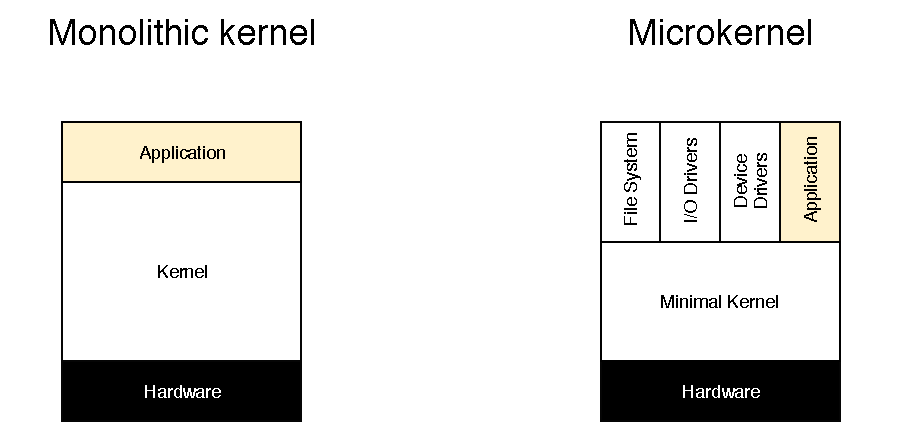
\includegraphics[scale=0.7]{assets/kernel_types.pdf}
    \caption{\label{fig:kernel-types}different kernel designs}
\end{figure}

% Others architectures
% Complete by mentioning other types?
Of course there are more architectures than what is listed above.
But in the context of this thesis, we considered that explaining in detail each one would not be relevant.
The two designs presented are the most common and provide a good preview of at what a kernel looks like.
Also, the following parts of this thesis will expand on this
    and we will see in practice what each RTOS uses from the theory.

\section{Scheduling}

The scheduler plays an important role in the design of a(n) (RT)OS.
The performances of an OS are deeply impacted by the scheduling algorithm it uses.
As we will see further in the thesis, it can also affect the energy consumption of the device.\\
%TODO reference for where

\subsection{Base concepts}

% What is a scheduler
A scheduler is a process designed to choose which task will run at a certain time in the system.
Different disciplines can be used, each one with multiple advantages and drawbacks.
Some commonly used are presented below in the Subsection 1.2.2.

% Preemptive vs non-preemptive (cooperative)
A scheduler is said to be \textit{preemptive} if tasks in the system can preempt each other.
When a higher-priority task wants to execute, the scheduler can interrupt a lower-priority task and run the higher-priority one.
In the other hand, a scheduler is said \textit{non-preemptive} or \textit{cooperative}
    if a task that has been allowed to start will execute until it is complete.

% online/offline
Another distinction we can make is to divide schedulers into \textit{online} and \textit{offline} schedulers.
% online
Online schedulers decide of the ordering of the different tasks during runtime based on various parameters (such as task priority for example).
A scheduler based on task priority is also called \textit{priority-based} scheduler.
% offline
On the contrary, offline schedulers (also known as \textit{table-driven} schedulers) perform their scheduling decisions at the start of the system.

The impact of these characteristics in the design of an RTOS will be explained later in this chapter.
%TODO reference

\subsection{Scheduling policies}

\subsubsection{First in, first out (FIFO)}
Also known as first come, first serve (FCFS), FIFO is one of the simpliest scheduling algorithm.
Processes are queued into a data structure in their order of arrival.
The first process to be enqueued is the first that will be executed.

\subsubsection{Round-robin}
The round-robin scheduling algorithm divides the time allocated to each process into fixed time slices.
If a process doesn not terminate when his allocated time slice is expired, the scheduler switches to another task.
If a task terminates within its time slice, the scheduler simply switches to the next task.

\subsubsection{Earliest deadline first (EDF)}
Earliest deadline first scheduling algorithm dynamically assigns a priority
    to each enqueued process (based on its deadline or an estimation of it) into a priority queue data structure.
The scheduler then executes the process the closest to its deadline at each scheduling event.

\subsubsection{Fixed-priority preemptive scheduling}
Priority for each task is pre-assigned by the operating system.
The scheduler arranges the tasks by order of priority.
Higher-priority tasks can interrupt lower-priority tasks.

%\subsection{Real-Time Scheduling}
%handbook chapter 2 12

\section{Memory management}

%https://www.memorymanagement.org/mmref/index.html#mmref-intro
%http://www.csc.twu.ca/rsbook/Ch12/Ch12.4.html
%https://www.gribblelab.org/CBootCamp/7_Memory_Stack_vs_Heap.html
%http://www.cs.virginia.edu/~son/cs414.f05/lec11.slides.pdf

In modern computer systems, memory management has evolved since early days techniques which were limited
    by early computer systems where each memory location was specified in the program.
This led to critical errors and/or unpredictability when an incorrect location was specified.

Nowadays, the memory management of (almost) every computer system follows the same principle:
the memory of a computer system can be divided into 2 distincts sections,
    the static memory (\textit{stack}) and the dynamic memory (\textit{heap}).

\subsection{Static memory management}
%stack
By the time a program begins to execute, there must be some specific blocks of memory reserved for its use.
This includes, for instance, the memory containing the program's own code.
Morever, every static variable must have a specific memory reserved.

The static memory allocation is predetermined by the compiler
    and will always be reserved for the program in the same manner at the beginning of every run.

This part of the memory operates as a \textit{stack} or last-in first-out (LIFO) queue.
The area of memory available for the use of the program will shrink and grow following the execution of the program,
which makes it very fast and efficient with no fragmentation.
%explain fragmentation?

\subsection{Dynamic memory management}
%heap
Sometimes, fixed memory size can be a problem.
Static memory does not allow allocation of memory beyond what is declared initially.
The \textit{heap} serves this purpose.
It is a large pool of memory which must be explicitly managed by the programmer.
It has no guarantee of efficient use of space, memory may become fragmented over time as blocks of memory are reallocated.

It may be tedious for the inexperienced programmer to manage the heap
    but it allows a more flexible and shareable pool of memory for an efficient programming.
To allocate memory on the heap, one must use \textit{malloc()} or \textit{calloc()} from the C code library stdlib.h (when available).
There are multiple algorithms to allocate memory when calling these functions.
The most common ones are presented below.

% conventional algorithms
\subsubsection{Sequential fit algorithm}
For this memory management algorithm, a single linkedvlist contains the unallocated blocks of memory.
When needed, they are allocated using different policies:
\begin{itemize}
    \item First fit: returns the first block large enough from the list.
    \item Next fit: similar to first fit but starts where the pointer was left off at the previous iteration.
    \item Best fit: research through the whole list and returns the smallest block large enough to meet the request.
    \item Worst fit: returns the largest block from the list.
\end{itemize}

\subsubsection{Buddy allocator algorithm}
This algorithm makes use of an array of linked lists.
Each list from the array owns blocks of a distinct size.
When requested, the buddy allocator algorithm finds the smallest but large enough block to meet the requirement from the array.
It then picks one of the block from this position in the array.

If the list is empty at the position where the best fitting block is located, it goes to the next position in the array
and splits a block from this list to fill the empty position.
The opposite can also be applied: two smaller blocks can be merged to obtain a bigger one.

\subsubsection{Indexed fit algorithm}
This algorithm makes use of an indexed data structure to implement the desired fit.
Some common data structures used for this algorithm are trees or hash tables.

\subsubsection{Bitmapped fit algorithm}
A bitmap representing the usage of the heap is created.
Each bit of the map corresponds to a part of the heap.
If a part is used, the bitmap is set to 1.
If not, it is set to 0.
Allocation is done by searching the bitmap for clear bits.

% unconventional algorithms?

%\subsection{Virtual Memory}
\section{Power management}

%to read
%https://dl.acm.org/citation.cfm?id=2333680
%https://dl.acm.org/citation.cfm?id=860179
%https://dl.acm.org/citation.cfm?id=860184
%https://ieeexplore.ieee.org/abstract/document/4054780
%http://www.es.mdh.se/pdf_publications/327.pdf
%https://www.sciencedirect.com/science/article/pii/S030626191630678X
%https://ieeexplore.ieee.org/abstract/document/5944309
%https://ieeexplore.ieee.org/abstract/document/8617010

%read
%https://www.sciencedirect.com/science/article/pii/S0167739X18329194


% \paragraph{}
% With the rise of cheap battery-powered embedded systems, the problem of energy efficiency becomes a non-negligeable stake.
% Each RTOS has its own way to manage its energy consumption.
% From a more general point of view, we can distinguish 2 ways to save energy in an embedded system.


% \subsection{Hardware energy management}

% At first, one could think that the hardware side of energy management is slightly out of context of the operating system means to save energy.
% The fact is that, even if we can distinguish 2 categories, the hardware means to save energy are very often tied to the upper layers of the whole system.

% \subsection{Software energy management}

The focus on energy management is something fairly recent in the field of information technology (IT).
With the rise of the Internet of Things (IoT), advancements have been made to allow operating systems to manage power consumption more efficiently.

Numerous communication stacks focused on IoT and low energy consumption have been developed in the last decade.
%TODO cite examples

Unfortunately lesser attention has been paid to the design of energy-efficient OS for resource-constrained devices.
Traditional hardware is limited in term of power management and the progress in this field required both software and hardware to evolve.
We will present below some of the advancements made and the technologies developed in recent years.


\subsection{Hardware power management}
In order to implement advanced techniques of power management, certain hardware features have been developed.
The purpose is to give more control from the software over the hardware.

\subsubsection{Clock gating}
% https://m.eet.com/media/1157354/fpmm%20-%20part%201.pdf
% https://en.wikipedia.org/wiki/Clock_gating
Clock gating is a technique consisting of turning off the clocks of unused peripherals in order to save energy.
Those peripherals enter what is called \textit{idle state} or \textit{sleep}.
The clocks are physically switched off from the circuit with the addition of a logical gate and do not consume energy until reactivation.

%power down mode? dynamic power
\subsubsection{CPU power down modes}
The recent advancements in CPU have introduced power-saving modes.
This feature stops the CPU clocks so that it is put to sleep unless
    a scheduling event or interrupt is triggered and wakes up the CPU, with the help of a real-time clock (RTC) for example.
% How the event can be scheduled if there is no clock to check the event ?

\subsubsection{Real-time clock wake up support}
% https://www.electronics-tutorials.ws/connectivity/real-time-clocks.html
When a CPU is in sleep mode, there is two possibilities to wake it up with an on-chip RTC or by an external event.
The on-chip RTC is a low-frequency clock (usually around 32kHz) that does not drain a lot of battery life.
RTC can include alarm functions: timers that when reached, trigger the RTC to wake up the processor.

\subsubsection{Supported CPU frequencies / dynamic frequency scaling}
In modern CPU, many options are available to switch between frequency ranges depending on the resources needed.
This feature can be used to minimize power consumption when  we do not need much computational power.

\subsubsection{Adaptive voltage scaling / dynamic voltage scaling}
%https://www.eetimes.com/document.asp?doc_id=1271842#
Similarly to the CPU frequency, voltage can be regulated based on the actual state of the chip.
The voltage is continuously monitored and adjusted during the runtime.


\subsection{Operating system power management}

\subsubsection{Peripherals state control}
Peripherals state control makes use of the clock-gating feature provided by the hardware.
Thanks to this feature, only the peripherals clocks required by the application at a certain point in time are active.
The other clocks are gated and do not consume energy.

\subsubsection{Sleep mode}
The idea is to allow the system to switch off certain components of the mi\-cro\-pro\-ces\-sor.

The sleep mode of a microprocessor takes advantage of multiple hardware features
    such as adaptative voltage scaling, CPU low-power modes and dynamic frequency scaling.
The RTC wake up support serves to wake up the CPU when in sleep mode and no other source is active.

\subsubsection{Tick suppression}
%https://www.embedded.com/electronics-blogs/industry-comment/4414162/1/FreeRTOS-s-tick-suppression-saves-power
Tick suppression defines the principle of providing tick-less support for the scheduler.

In a regular scheduler, a periodic timer (tick interrupt) is used to track time.
This tick interrupt wakes up the CPU to perform a scheduling cycle.
Such a mechanism, even if punctual, is frequent and then depletes power in a non-negligeable way by entering and exiting sleep mode frequently.

In a tick-less scheduler, the tick interrupt is disabled when the idle task is running.
Stopping the tick interrupt allows the CPU to remain in a deep power-saving state 
    until either an interrupt occurs or it is time for the kernel to switch task.

%schema tick vs tickless scheduler
\section{Programming model}
%definition
The programming model of an RTOS can be seen as "the way to program" an application using a specific RTOS.
Different "ways to program" or paradigms are predominant in the world of RTOS.
In this section, we will present the two main different paradigms used\cite{comparison_iot_constrained_devices}.


\subsection{Event-driven model}
In an event-driven programming model, a program generally consists of a main loop which listens for events.
Events can be generated by interrupts, sensors or user input.
When an event is detected, a callback function is triggered.

The developper has to manually maintain state across tasks which can be tedious.
Thus, the individual tasks do not have to maintain their own stack and they use a shared stack.
The memory footprint is then reduced since a single stack is used across the application.

\subsection{Multithreaded model}
The multithreaded model allows an application to run different tasks in their own thread context,
    and communicate between them using an IPC API.

Each thread has its own memory stack and does not require manual management by the programmer.
The stack is managed automatically by the thread scheduler.
The memory requirements of threaded application are often larger than their event-driven counterparts.
\section{Hardware support}

The embedded world is responsible for the majority of the world's microcontrollers.
The diversity of CPU keep increasing every year.
Working with this diversity of constrained devices makes the developer's work harder as he needs to adapt and learn to use specific librairies for each devices.
A source code on a particular device will not be easily reusable for another device.

With RTOS, developers can more easily make their code portable on many devices.

This section first describes the three constrained devices classes and how this is related to RTOS.
Then, it explains what an hardware abstraction layer (HAL) is and how a RTOS uses it in order to be compatible with the largest amount of devices.

\subsection{Constrained devices classes}

Constrained devices have been classified in 3 classes by the Internet Engineering Task Force (IETF) with the request for comments RFC7228 in May 2014.
%TODO cite rfc
IETF is a standards organization aiming at improving and maintaining the usability of the Internet.
Therefore they play a certain role in the evolution of IoT technologies.
We can argue that IETF is a competent authority over constraints devices since its domain of competence is the Internet.
Nonetheless, the boundary between constrained embedded devices and the Internet is permeable.
For the purpose of this thesis, the classification they made with RFC7228 is used.
RFCs are informational or experimental documents published by engineers and computer scientists.
Some of them become standards and some others \textit{de facto} standards.

The distinction between the three classes are made with the random-access memory (RAM) and read-only memory (ROM) capabilities of each device.
Table \ref{tab:constrained-devices-classes} resumes the different constrained devices classes.

\begin{table}[!h]
  \centering
  \begin{tabular}{|l|l|l|}
  \hline
   & Data size (e.g., RAM) & Code size (e.g., flash) \\ \hline
  Class 0 (C0) & \textless{}\textless{} 10 kB & \textless{}\textless{} 100 kB \\ %\hline
  Class 1 (C1) & $\sim$ 10 kB & $\sim$ 100 kB \\ %\hline
  Class 2 (C2) & $\sim$ 50 kB & $\sim$ 250 kB \\ \hline
  \end{tabular}
  \caption{classes of constrained devices}
  \label{tab:constrained-devices-classes}
\end{table}

\paragraph{Class 0.}
Those devices are the most constrained.
There are typically sensor nodes (or motes) in a sensor network.
There are so constrained that they cannot access Internet without the help of a larger devices.
The source code of a RTOS is often too heavy to fit in such devices.
Instead Class-0 devices are usually used bare metal.
In the embedded world, bare-metal programming is writing code that runs directly on the hardware without any abstraction such as an OS.

\paragraph{Class 1.}
Those devices are able to talk to each other but via constrained protocols.
The use of security protocols are often too heavy for that class.
%RTOS mainly target this kind of devices.
RTOS generally require at least a few kB for the strict minimal functionalities to run.
Therefore, they are not practical for class 0 devices (even if they could technically run) and mainly target class 1 or more powerful devices.


\paragraph{Class 2.}
Those devices are the less constrained and can use the same stacks of protocols used in personal computers and servers.
General-purpose OS can be used for this kind of devices but the class-2 devices can benefit from lightweight and energy-efficient protocols.

\subsection{Hardware abstraction layer}

Due to the variety of CPU, vendors provide a set of libraries used to develop applications on their architectures.
This set of libraries and tools are called the hardware abstraction layer.

\paragraph{Definition of HAL}
% TODO
% Repetition of 'hardware'
A hardware abstraction layer defines a set of routines, protocols and tools to access underlying hardware.
It provides abstract and high-level functions to interact with the hardware.
The hardware, drivers and board supports are considered as black-boxes.

\paragraph{RTOS and HAL}
The HAL is strongly dependent on the architecture of the CPU.
In order for the RTOS to support multiple boards and architectures, it has to implement and use the different HAL provided by the vendors.

\begin{figure}[!h]
  \centering
  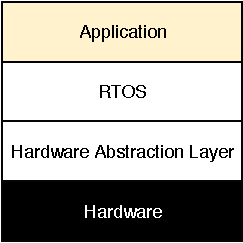
\includegraphics[scale=1]{assets/hal-layers.pdf}
  \caption{\label{fig:hal-layer}layers around the hardware abstraction layer}
\end{figure}

Figure \ref{fig:hal-layer} shows that the application and RTOS layers are placed above the HAL, itself just above the device layer.
The application layer talks to the RTOS and the RTOS layer talks to the corresponding HAL depending on the device used.

%TODO rework this part
\paragraph{Pro and cons}
Developers can switch hardware and perform cross-platform testing more easily.
But there is some limitation: the HAL is tied to the hardware and change heavily with it.
Also, there is some limitation using an hardware abstraction layer.
Not all the functionalities from the hardware are available.




%%%%%% Chap 2 %%%
\chapter{RTOS outline}

In this chapter, we will cover the specificities of each OS we planned to work with.
We chose to write about technical and non-technical characteristics of the chosen OS and even their respective projects as a whole.

%Some of the things written in this chapter are personal opinions.
%Indeed, as we decided to include non-technical characteristics of each of the projects, some subjectivity is involved.
%We tried to be critical and impartial in those points but it beware it only reflects our own opinions.

A table summarizing the comparison is provided at the end of the chapter.

%https://www.simform.com/iot-rtos-selection/
%https://ijarcce.com/wp-content/uploads/2015/12/IJARCCE-92.pdf
%http://www.ipcsit.com/vol1/54-S028.pdf

%Supported Architecture
%License
%User-friendly/documentation/example applications
%Supported network protocols
%kernel type
%date of creation
%file systems supported
%number of boards supported
%memory footprint
%resource access control (posix...)
%memory management policy
%energy management features
%programming model
%scheduling
%community
%build system
%ipc management

\section{RIOT}
%TODO explain why we chose riot

\subsection{Historic}

The RIOT project started privately in 2008.
It started as a part of the FeuerWhere project (\url{http://feuerwhere.mi.fu-berlin.de}), 
    where firefighters would be tracked with embedded devices during an intervention.
The goal was to design an ad hoc self-configurating network of sensors used 
    to monitor vital state and environmental parameters of rescue forces inside a building.

% https://ieeexplore.ieee.org/stamp/stamp.jsp?tp=&arnumber=6142316
In 2010, a fork from the FeuerWare software developed for the FeuerWhere project was made.
Development continued for $\mu$kleos\cite{microkleos}, a microkernel-based operating system for embedded devices.
The focus of this system was modularity and Internet compliance with the integration of IETF protocols such as 6LoWPAN, RPL and TCP.

In 2013, RIOT went public.
$\mu$kleos was rebranded to avoid problems with spelling and pronunciation.
Since then, more than 200 people contributed to the project with more than 20 000 commits and 75 releases.
The project is currently supported by Freie Universität Berlin, INRIA and Hamburg University of Applied Sciences.

\subsection{Characteristics and features}
%ce que fait l'os
%https://www.osrtos.com/rtos/riot/
RIOT is an open-source real-time operating system.
The OS provides a lightweight operating system with multithreading and real-time features running across a wide range of resources constrained devices.
It runs on 8-bit, 16-bit and 32-bit platforms and only needs a minimum of 1,5 kB of RAM.
A focus has been made on making RIOT standard-C and C++ compliant.

\paragraph{License} RIOT is distributed under the LGPL2.1 license which provides unrestricted commercial or private use, modification and distribution if it is not a derivative work.
With LGPL license, RIOT is also provided "as is", without any warranty of any kind.

\paragraph{Technicals} The RIOT project aims to bridge the gap between operating systems for Wireless Sensor Networks (WSN) and traditional fully fledge operating systems.
RIOT follows some design objectives such as:
\begin{itemize}
    \item Energy efficiency
    \item Small memory footprint
    \item Modularity
    \item Uniform API, platform agnostic
\end{itemize}

%https://github.com/RIOT-OS/RIOT/wiki/RIOT-Community-Processes
\paragraph{Community} The RIOT community can be characterized in 3 categories\cite{RIOTComm}:
\begin{itemize}
    \item Contributors are people who contributed to the project, from code contribution to technical or non-technical discussions.
    \item Maintainers who contributed noticeably on the project.
        Maintainers can propose to give the maintainer status to contributors that have been noticed.
        The status comes with rights (merge rights) and duties (code review duties).
    \item Coordinator status is acquired following the same principle as the maintainer.
        The role covers non-technical aspects of the project such as bringing up topics, debates and deal with the overhead.
\end{itemize}

\subsection{Specificities}
%https://hal.inria.fr/hal-00768685v1/document
%static memory for the kernel
%dynamic memory
RIOT enforces constant time for kernel tasks.
The kernel exclusively uses static memory which guarantees runtimes of \textit{O}(1) whereas dynamic memory is used for applications.

The scheduler cycle is also performed in constant runtime thanks to a circular linked list of threads\cite{riotspec}.

%tickless
The main specificity of RIOT resides in its scheduler.
The operating system includes a tickless scheduler.
When there is no pending task, the operating system will switch to the \textit{idle} task which is the thread with the lowest priority.
The CPU will then put itself in its deepest possible sleep mode (which depends on the device in use).
In this state, the device can only be woken up by an interrupt (external or kernel-generated).
\section{Contiki}
%https://komalbattula.wordpress.com/architecture/
%explain contiki and why we chose it

\subsection{Historic}
%https://ieeexplore.ieee.org/stamp/stamp.jsp?tp=&arnumber=1367266
%https://ercim-news.ercim.eu/en76/rd/contiki-bringing-ip-to-sensor-networks
Contiki was created in 2003 by Adam Dunkels. %http://dunkels.com/adam/
At the time, it was the first operating system to provide IP connectivity to sensor networks.
It did so thanks to $\mu$IP, a lightweight TCP/IP stack intended for tiny microcontrollers,
    also developped by Adam Dunkels at the Swedish Institute of Computer Science (now RISE SICS).%https://github.com/adamdunkels/uip

Further developpement of Contiki has been supported by various industries and research institutes 
    such as Texas Instruments, Atmel, Cisco, ENEA, ETH Zurich, Redwire, RWTH Aachen University, 
    Oxford University, SAP, Sensinode, Swedish Institute of Computer Science, ST Microelectronics and Zolertia.
%death?

\subsection{Characteristics and features}
The developpement of Contiki started with the need to bring connectivity to small sensor devices with limited capabilities.
By definition, Contiki is not a real-time operating system and has not been designed as such.\\

%memory allocation/stack and kernel/event driven
Contiki operates with the event-driven model.
Processes are implemented as event handlers that run to completion.
An event handler can be defined as a procedure that performs a specific action in response to an event.
Because event handlers cannot block, the same stack can be shared among them.
Also, locking mechanisms are not needed as event handlers do not run concurrently.
Instead of having multiple stacks for multiple threads (which must be over-provisioned or they risk to run out of memory), a single stack can then be used.

This model does not come without problems, as it is sometimes tedious for programmers to manage.
For example, a time-consumming process such as a cryptocraphic operation can monopolize the CPU for quite some time 
    and make the system unable to respond to external events. 
In a preemptive multi-threading system, the computation can be preempted to react to an external event 
    and continue the process later.
To fix this issue, Contiki makes use of an application library that implements preemptible threads.
This library is optional an can be used with programs that explicitly require it.\\

%protothreads
%http://dunkels.com/adam/dunkels05using.pdf
In order to implement its event-driven system, Contiki comes with a mechanism called \textit{protothread}.
The concept of protothreads was also developped by Adam Dunkels with the help of other researchers.
The goal of the protothread programming abstraction is to make it easier for developpers to develop, debug and maintain code written in the event-driven model.

Protothreads can be defined as lightweight stackless threads providing a blocking context on top of an event-driven system.
They can be used to perform non-preemptive concurrency or cooperative multitasking.
Programs written for an event-driven model typically have to be implemented as explicit state machines.
With protothreads, programs can be written in a sequential fashion without designing explicit state machines.

Protothreads do not serve the same purpose as threads for the event-driven model.
The concept has been developped to bring a number of benefits of the multi-threaded programming model into Contiki
    and ease the developpement of applications.\\

%energy saving mechanisms
Contiki does not provide any specific kernel energy saving mechanism.
Instead, it let the application specific parts of the system implement such mechanism.

\subsection{Specificities}
%contiki is specific by itself, aims for WSN
%dynamic loading? is that necessary to develop that?
%cooja
Contiki integrates a tool called Cooja.
Cooja is a network simulator which is designed to simulate a network using Contiki motes.
Motes can be simulated at the hardware level or with a standard setup allowing faster response but with less precise system behaviour.
It is an extremely powerful tool which makes developping and debugging tremendously easier even with a large-scale network.

\begin{figure}[!h]
    \centering
    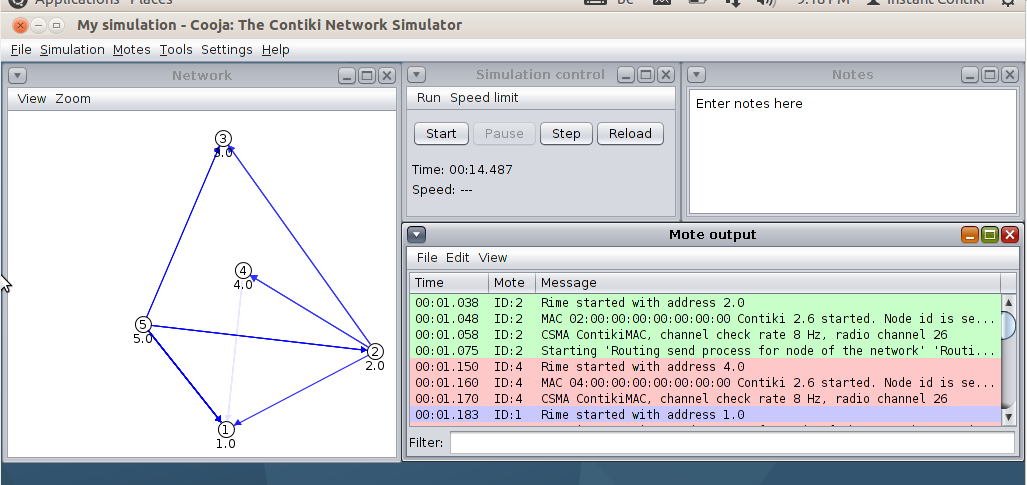
\includegraphics[scale=0.4]{assets/cooja.png}
    \caption{\label{fig:cooja}Cooja interface}
\end{figure}

%rime https://pdfs.semanticscholar.org/9feb/7e0f0d3b507f2f3da60c1b2fea9d5e43449d.pdf
%Contiki provides a low-power radio networking stack called Rime.
%This stack can be used where the full IP stack is not needed.
%The Rime stack can be tuned to 
\section{FreeRTOS}

\subsection{Historic}
\paragraph{}
%https://www.freertos.org/RTOS.html
The FreeRTOS kernel has been developped in 2003 by \href{https://www.linkedin.com/in/richard-barry-4562262/}{Richard Barry}. %fix href pls
He founded a company called Real Time Engineers Ltd to develop and maintain FreeRTOS until the stewardship of the project was passed to Amazon Web Services in 2017.
Since then, we can distinguish the FreeRTOS kernel and Amazon FreeRTOS which includes the aforementioned kernel 
    with a set of libraries extending the functionalities of the RTOS.

\subsection{Characteristics and features}
\paragraph{}
%real time
Similarly to RIOT OS, FreeRTOS is designed to be a real-time preemptive operating system aimed at embedded devices.
Its strength comes from the fact that it is highly and easily configurable.\\

%scheduler
%http://richardgoyette.com/Research/Papers/FreeRTOSPaper.pdf
For example, FreeRTOS supports preemptive or cooperative scheduling. 
It also uses Dynamic Priority Scheduling which means that the priorities are defined during runtime.
The user can choose which scheduling policy he wants by modifying the \texttt{configUSE\_PREEMPTION} variable in the \texttt{FreeRTOSConfig.h} file.
In the cooperative case, the only action the scheduler performs is to increase the tick count.
In the preemptive case, the scheduler increments the tick count and then checks if a task is in the unblocked state.
If it is indeed the case, it checks the priority level of the task and compares it with the current task to see if a switch is required.\\

%tasks and coroutines
%https://www.freertos.org/taskandcr.html
%https://www.researchgate.net/profile/Ming_Yuan_Zhu/publication/308692183_Understanding_FreeRTOS_A_Requirement_Analysis/links/57eb301108ae5d93a4816184.pdf
Since FreeRTOS uses the multi-threading paradigm, the code can be structured as a set of tasks.
As explained in the first chapter, each task use its own stack and therefore has its own context.

In addition to tasks, FreeRTOS includes a another mechanism called \texttt{co-routine}.
Co-routines are similar to tasks but have some fundamental differences which justify their usage:
\begin{itemize}
    \item They share the same stack between them which greatly decrease the memory wasted in provisioning.
    \item They use a cooperative scheduling between them but they can be used in an application using preemptive tasks.
    \item The shared stack comes with more restrictions on how co-routines can be structured compared to regular tasks.
\end{itemize}
Co-routine have been implemented for very RAM constrained devices and are very rarely used those days.
Nonetheless, they stay a relevant alternative to tasks for specific usages.\\
%ipc
%deadlock avoidance
%scheduler suspension
FreeRTOS also supports tickless idle mode, similarly to RIOT.
Since FreeRTOS is highly configurable, the developer can activate this feature 
    by setting the variable \texttt{configUSE\_TICKLESS\_IDLE} as 1 in \texttt{FreeRTOSConfig.h}.
A custom built tickless idle mode can also be provided by the developer and used by setting the same variable to 2.
This feature can be used when a default implementation in not provided for a certain board.
%memory allocation
\section{Comparison Table}

\part{Implementing a benchmarking framework in the context of a RTOS}
%%%%%% Chap 3 %%%
\chapter{Objective}

% TODO
% Add a introduction text here...

\section{Implementing a benchmarking framework}

% https://www.electronicdesign.com/embedded/11-myths-about-embedded-benchmarking

The first question one can ask is "What does benchmarking an embedded system means?".
A benchmark measures the performances of a defined system, in our case, an embedded system.
Those performances can be measured in terms of latency, memory usage or even energy consumption.
But we can also see benchmarks that include reliability, interoperability or stability measurements.
In the scope of our thesis, we chose to only focus on latency measurements.

In order to assess the performances of an application deployed on a RTOS, we wanted to build a benchmarking framework.

\subsection{Motivations}

In the RTOS world, benchmarks already exist and some of them are even commercialized.
% https://grahn.cse.bth.se/Papers/ParMiBench_crc.pdf -> ParMiBench
% http://vhosts.eecs.umich.edu/mibench//Publications/MiBench.pdf -> MiBench
% https://pure.tue.nl/ws/portalfiles/portal/46936147/640318-1.pdf
% TODO - Donner des exemples de benchmarking
However, those benchmarks are just workloads.
They use a defined set of routines that is used to measure the performances of a RTOS.
This does not reflect the performances of a real-world application.
A benchmark must be a tool that a developer can use to have a fair comparison of two systems.

Developers find themselves using other tools to assess the performances of their applications.
Let's take for example, the case of a developer who want to measure the latency of its application.
A benchmark will only provide a latency measurement based on predefined tasks and within a controlled environment.
If our developer wants to measure the real latency of its application, he will need to use an oscilloscope and take the time to do the measurements.

However, this kind of devices is costly and some developers can not afford them.
Furthermore, working with external devices takes time and can dramatically slows down the development process.

For those reasons, we wanted to build a benchmarking framework hidden from the developer that he could run on any RTOS with any application.

Ideally, the use case for any developer using our benchmarking framework would be the following.
This scenario is hypothetic and does not represent the state of our work.
The developer implements an application with multiple tasks on a specific device.
The developer wants to measure the performance of its application and, to do so, set a flag in the Makefile of its application to turn on the benchmarking framework.
The developer flashes its application on the device and the framework output continuously performance measurement of the application.
With this framework, the developer can optimize its application or change the device and check if the context switching time is improved.

\subsection{Criteria}

Ideally, this framework would respect the following criteria in order to be useful for a real-world application.

\paragraph{Widely distributed}
By making our framework accessible on a large variety of RTOS, we allow developers not to limit themselves to a specific set of RTOS.
With this framework, they would be able to assess the performance of their applications regardless of the platform.

\paragraph{Providing a large variety of metrics}
Our framework should be able to provide performance measurements on interrupt latency, context switching time.
Those metrics are important for a real-time context applications.
Also, using constrained devices requires to monitor the memory usage and the energy consumption of the applications.
Our framework should be able to provide those metrics as well.

\paragraph{Hidden for the developer}
The developer should not need to worry about integrating our framework in its application.
Using or not our framework should not change the source code of the application and allow the developer to directly deploy it in a production environment.

\paragraph{Easy to use and to configure}
Using an oscilloscope or any external device to benchmark an embedded application takes time and effort for the developer.
Our framework should be able to improve the benchmarking process by being easy to use and easy to configure.

\subsection{Approaches}

In order to develop this framework, we explored in three different approaches.
We introduced them here so that the reader have already in mind our three experiments but each one of them is described later in the chapter \ref{chap:experiment}.

\paragraph{Integrating the framework in the kernel of the RTOS}
Our first approach was to integrate the framework in the heart of the RTOS.
By focus our implementation in the kernel space, we would be able to retrieve performance measurements without altering the user space and the application.
This approach is detailed in the section \ref{sec:kernel}.

\paragraph{Implementing the framework as an extension of the RTOS}
The majority of RTOS allow user to develop their own extension without altering the kernel source code.
We choose to investigate this opportunity with our second approach.
The framework would be an extension of RTOS.
This implementation is explained in the section \ref{sec:extension}.

\paragraph{Using external devices}
Finally, our last approach was to use external devices such as the computer or an external board to benchmark our real-world application.
This last idea is described in the section \ref{sec:external}.

\section{Narrowed objective and limitations}

Building a complete benchmarking framework is an ambitious work that requires a lot of time.
In the scope of our thesis, we chose to narrow down our objective and produce only a proof-of-concept.
By implementing this proof-of-concept framework, we want to show that it is possible to build a large benchmarking framework given more time and effort.

For our proof-of-concept, we have reduce our framework implementation to a benchmarking of the context switching time RTOS that use a cooperative scheduler.
From the criteria previously described, we have decided to reduce the first two by focusing only on a specific set of RTOS and the context switching time.
For the last two, we leave them untouched in order to build a benchmarking framework the most hidden and easy-to-use for the developer.

We left the goal to implement a framework capable of benchmarking the interrupt latency, the memory usage and the energy consumption of any RTOS to future work.

\subsection{Context-switching time centric framework}

We chose to focus on the context switching time for the metric of our benchmarking framework because, in the context of embedded devices, the time spent between two tasks must be the smallest possible.
Benchmarking the context switching time can help the developer to reduce the time lost between two tasks.
Moreover, by considering the interrupt handler as a task, it is possible to compute the interrupt latency with the context switching time.

\subsection{Scheduler limitations}

We chose to only use RTOS with cooperative scheduler because this kind of scheduler allows us to know when a task is in the foreground and when it goes to the background.
With a preemptive scheduler, in the other hand, we do not know when the task is preempted.

% For that reason, we chose to focus our work on two RTOS: Contiki and FreeRTOS.

For example, in Contiki, the developer can use macros like \texttt{PROCESS\_PAUSE()} or \texttt{PROCESS\_WAIT\_EVENT()} to let other tasks run in a cooperative fashion.
% https://github.com/contiki-os/contiki/wiki/Processes
The complete list of macros and more information can be found in the \href{https://github.com/contiki-os/contiki/wiki/Processes}{Contiki processes documentation}.

RIOT OS, in the other hand, uses a preemptive scheduler.
But it is possible to implement an application in a cooperative fashion.
By defining the tasks priorities at the same value, it is possible to call \texttt{thread\_yield()} to provoke a context switch.
More information can be found in the \href{https://riot-os.org/api/group__core__sched.html}{scheduler documentation} of RIOT OS.

For those reasons, we chose to focus our work on these two RTOS: Contiki and RIOT OS.
\section{Reference value}

Our benchmarking framework will compute the context switching time but we need to know how well or how bad our framework performs.
To assess the performance of our measurements, we first need to compute the real context switching time.
This real context switching time will be our reference value.

\subsection{Simple application}
In order to experiment and test our benchmarking framework, we need to have a simple application on every tested RTOS.

The application contains two indentical tasks.
The tasks wait for 1ms in the foreground and then goes to the background letting the scheduler runs the next task.
The tasks run in an infinite loop.

\subsubsection{Implementation in Contiki}
The source code of one of the two tasks is shown in the listing \ref{lst:simple-task-code}.
It uses the \texttt{clock\_delay\_usec()} call to make the task wait for 1ms.
Finally, we use the \texttt{PROCESS\_PAUSE()} macro to pause the task and let the other task do its iteration.

\begin{lstlisting}[style=CStyle, float, label={lst:simple-task-code}, caption={Source code of a task implemented in Contiki for the simple application}]
PROCESS_THREAD(task, ev, data)
{
    PROCESS_BEGIN();

    while (1)
    {
        clock_delay_usec(1000);
        PROCESS_PAUSE();
    }

    PROCESS_END();
}
\end{lstlisting}

\subsubsection{Implementation in RIOT OS}
The source code of on of the two tasks is shown in the listing \ref{lst:simple-task-code-riot}.
We can not use the \texttt{xtimer\_usleep()} method as it will lead to a context switch.
Instead, we used a for loop.
The \texttt{thread\_yield()} call will perfom a context switch and let the other task run on iteration.

\begin{lstlisting}[style=CStyle, float, label={lst:simple-task-code-riot}, caption={Source code of a task implemented in RIOT OS for the simple application}]
void *threadA(void *arg)
{
    (void)arg;

    while (1)
    {
        for(int i = 0; i < 1000; i++) {}
        thread_yield();
    }
    return NULL;
}
\end{lstlisting}


\subsection{Methodology}

In order to compute the real context switching time, we used an oscilloscope and two GPIOs.
Each task of our simple application is responsible of one GPIO.
Every time a task is run and goes to the foreground, it sets its GPIO up.
Once the task is finished and goes to the background, it resets its GPIO down.

With the oscilloscope, we can mesure the voltage of the two GPIOs and compute the real context switching time from those measurements.
The figure \ref{fig:real-context-switching-time-measurement} shows the different steps of our methodology.
On this schema, the execution time of the two tasks are represented above the voltage measurements of the two GPIOs.
The context switching time happens between the execution of the two tasks and is bordered with dotted lines.

\begin{figure}[!ht]
  \centering
  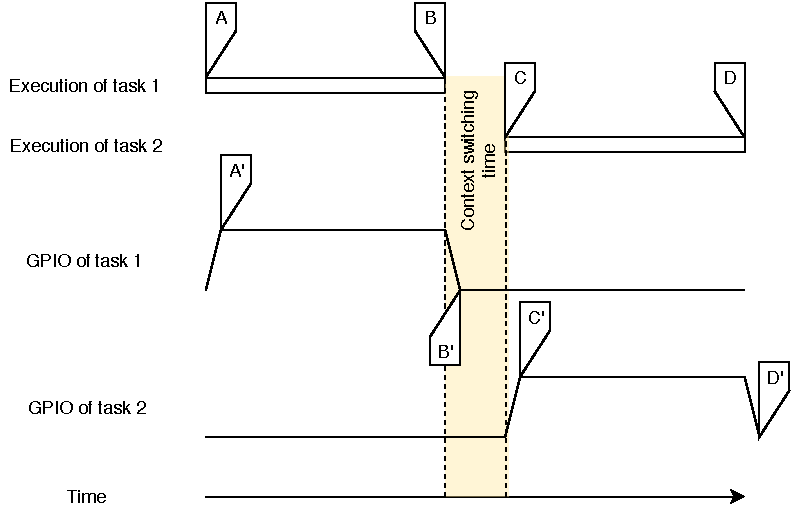
\includegraphics[scale=1]{assets/real-context-switching-time-measurement.pdf}
  \caption{\label{fig:real-context-switching-time-measurement}Steps in the methodology to compute the real context switching time}
\end{figure}

The steps are the following.
The first task sets up its GPIO on step A.
The GPIO is in high position few nano seconds later on step A'.
Once the first task is over, it resets its GPIO on step B which goes in low position on step B'.
In the same way, the second task set up its GPIO on step C which goes in high position on step C' few nano seconds later and reset it on step D which goes in low position on step D'.
The oscilloscope measures the context switching time between the step B' and the step C'.
The time for the GPIOs to rise up or down are around 10 nano seconds and can be omitted.


\subsection{Measurement setup}

The oscilloscope used for the measurement was the \href{https://www.tek.com/oscilloscope/mso56}{Tektronix MSO 56} available at the Welcome Lab at UCLouvain.
We used two channels to measure the voltage of the two GPIOs used by the application.
The interface of the oscilloscope, shown in the figure \ref{fig:oscilloscope-interface}, allows us to directly see in real-time our measurements.
A table resume the measurements displayed in the graph below while we can check the voltage of our two GPIOs in the bottom-right window.
Once we have retrieved 1000 measurements, we export our data in a flash thumb.

\begin{figure}[!ht]
    \centering
    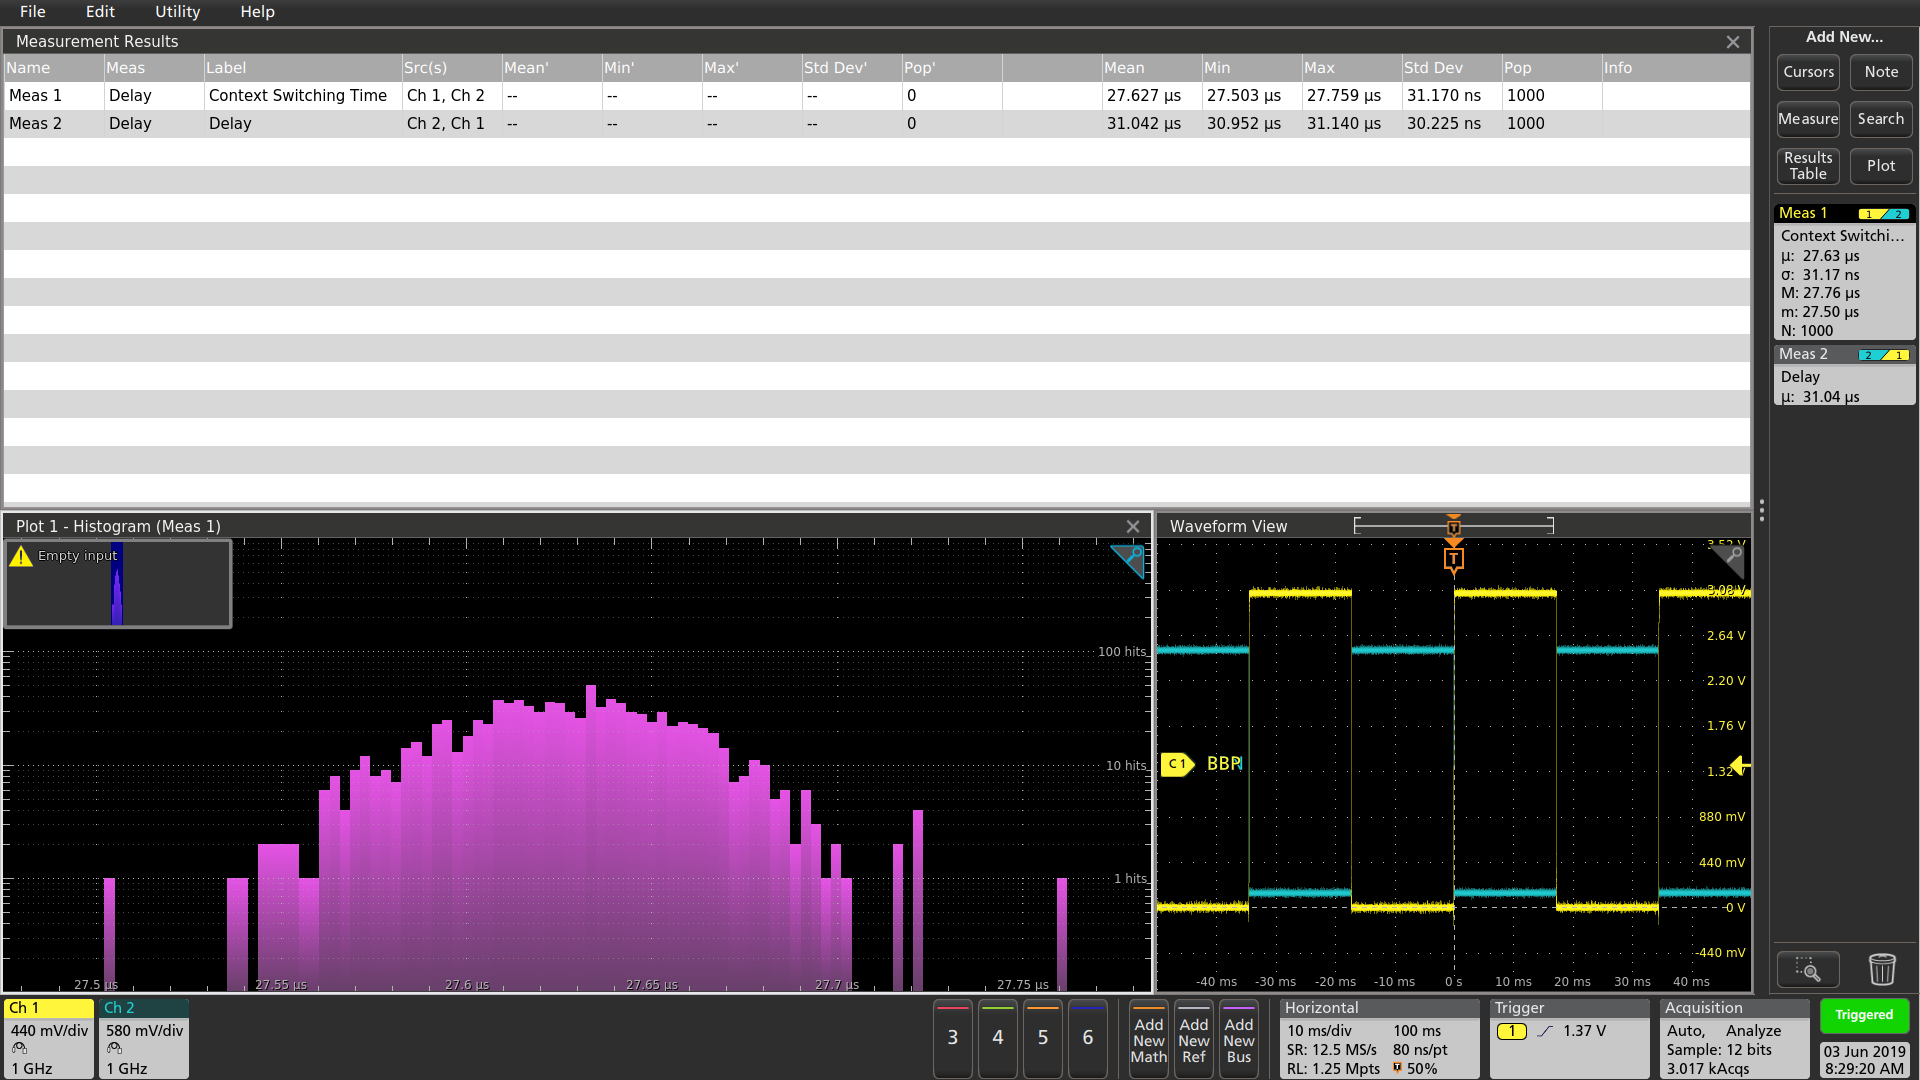
\includegraphics[scale=0.25]{assets/oscilloscope-interface.png}
    \caption{Interface of the oscilloscope\label{fig:oscilloscope-interface}}
\end{figure}

We updated our simple task by adding GPIO calls in order for the oscilloscope to detect it.
The task will set up a GPIO, wait for 1ms, and then clear the GPIO.
The two tasks use different GPIO in order to differenciate them with the oscilloscope.

\subsubsection{Implementation in Contiki}
The source code of the updated task is shown in the listing \ref{lst:gpio-task-code}.
\texttt{GPIO\_SET\_PIN()} and \texttt{GPIO\_CLR\_PIN()} are used to respectively set and clear the GPIO used by the task.

\begin{lstlisting}[style=CStyle, float, label={lst:gpio-task-code}, caption={Source code of the task with GPIO calls}]
  PROCESS_THREAD(task, ev, data)
  {
      PROCESS_BEGIN();
  
      while (1)
      {
          GPIO_SET_PIN(
              GPIO_PORT_TO_BASE(GPIO_C_NUM), 
              GPIO_PIN_MASK(3));

          clock_delay_usec(1000);

          GPIO_CLR_PIN(
              GPIO_PORT_TO_BASE(GPIO_C_NUM), 
              GPIO_PIN_MASK(3));

          PROCESS_PAUSE();
      }
  
      PROCESS_END();
  }
\end{lstlisting}

\subsubsection{Implemetation in RIOT OS}
The source code of the updated task is shown in the listing \ref{lst:gpio-task-code-riot}.
\texttt{gpio\_set()} and \texttt{gpio\_clear()} are used to respectively set and clear the GPIO used by the task.

\begin{lstlisting}[style=CStyle, float, label={lst:gpio-task-code-riot}, caption={Source code of a task implemented in RIOT OS for the simple application}]
    void *thread(void *arg)
    {
        (void)arg;
    
        while (1)
        {
            gpio_set(GPIO_PIN(PORT_C, 2));

            for(int i = 0; i < 1000; i++) {}

            gpio_clear(GPIO_PIN(PORT_C, 2));

            thread_yield();
        }
        return NULL;
    }
    \end{lstlisting}

\subsubsection{Boards used}

To perform our measurements, we have used two devices from Zolertia.
The \href{https://github.com/Zolertia/Resources/wiki/RE-Mote}{RE-Mote} and the \href{https://github.com/Zolertia/Resources/wiki/The-Z1-mote}{Z1}.
The CPU of the RE-Mote is a \href{https://developer.arm.com/ip-products/processors/cortex-m/cortex-m3}{ARM Cortex-M3} 32 MHz clock speed with 512 KB flash and 32 KB RAM.
The Z1 have a \href{http://www.ti.com/product/MSP430F2617}{MSP430F2617} 16 MHz clock speed with 92KB flash and a 8KB RAM.

With those specifications, the Zolertia RE-Mote categorizes itself as a Class 2 device and the Zolertia Z1 as a Class 1 device.
Moreover, both Contiki and RIOT OS support those boards.

\begin{figure}[!ht]
    \begin{minipage}{.45\textwidth}
        \centering
        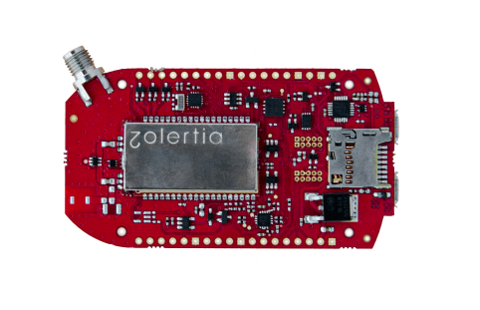
\includegraphics[scale=.5]{assets/remote.png}
        \caption{Zolerta RE-Mote board}
    \end{minipage}\hfill
    \begin{minipage}{.45\textwidth}        
        \centering
        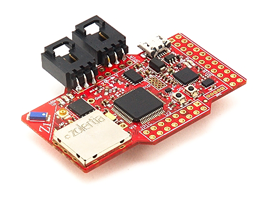
\includegraphics[scale=2.5]{assets/z1.png}
        \caption{Zolerta Z1 board}
    \end{minipage}
\end{figure}

\subsection{Measurement results}

In the end, we have four differents reference values.
One for each board and for each RTOS.
The results are divided by boards and the measurements from Contiki are compared side-by-side with the measurements from RIOT OS for more clarity.

\subsubsection{RE-Mote measurements}
With the RE-Mote board, we have measured an average context switching time of $18.505\mu s$ for Contiki and $12.626 \mu s$ for RIOT OS.
The table \ref{tab:reference-value-remote} shows the statistics of the measurements.

\begin{table}[!ht]
  \centering
  \begin{tabular}{l|c|c}
       & Contiki & RIOT \\ \hline
  Mean ($\mu$s) & 18.505 & 12.626 \\
  Min  ($\mu$s) & 14.312 & 12.549 \\
  Max  ($\mu$s) & 72.753   & 12.656
  \end{tabular}
  \caption{Reference value for Contiki and RIOT on the RE-Mote}
  \label{tab:reference-value-remote}
  \end{table}

The figure \ref{fig:reference-value-contiki-remote} and the figure \ref{fig:reference-value-riot-remote} show the distribution of the reference value with the RE-Mote board.
Note that the y-axis is logarithmic.
For the reference value of Contiki, we can see that the majority of the measurements is around $14 \mu s$.
Some measurements are above $35 \mu s$ with extrema around $70 \mu s$.
For RIOT, we find two distributions.
One around $12.56\mu s$ and the other around $12.64\mu s$.

\begin{figure}[!ht]
    \begin{minipage}{.45\textwidth}
        \centering
        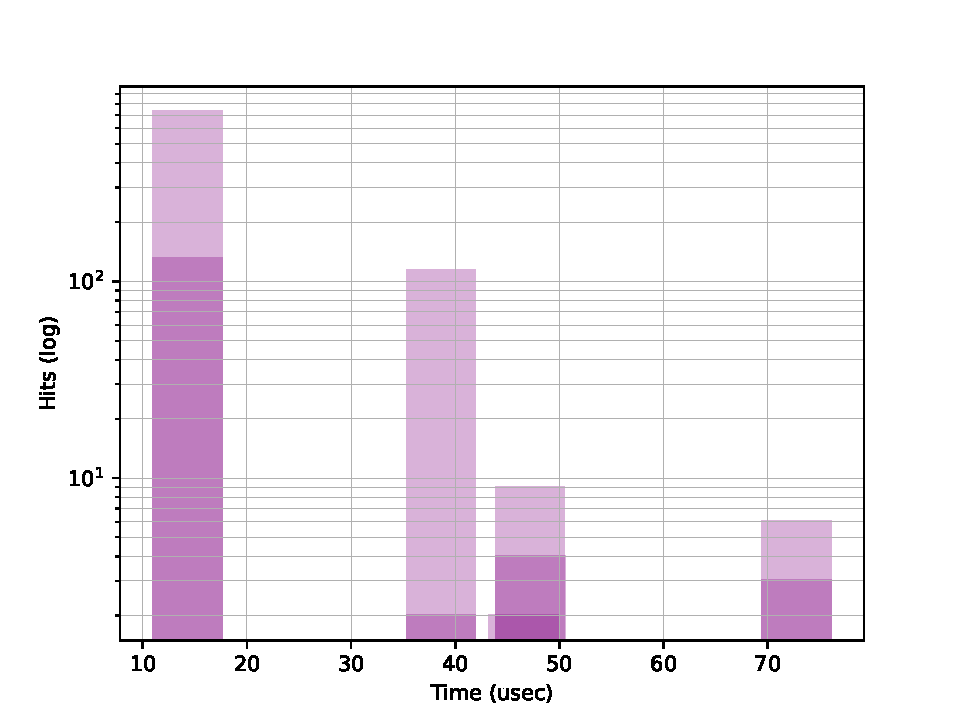
\includegraphics[scale=.4]{assets/reference-value-contiki-remote.pdf}
        \caption{Reference value distribution with Contiki on RE-Mote\label{fig:reference-value-contiki-remote}}
    \end{minipage}\hfill
    \begin{minipage}{.45\textwidth}        
        \centering
        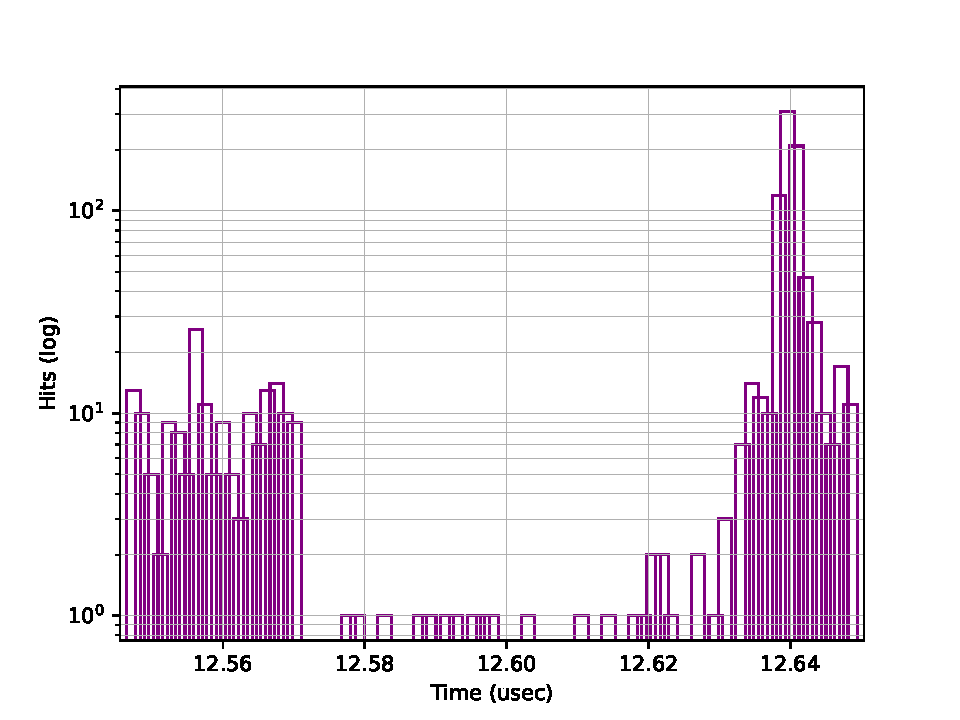
\includegraphics[scale=.4]{assets/reference-value-riot-remote.pdf}
        \caption{Reference value distribution with RIOT OS on RE-Mote\label{fig:reference-value-riot-remote}}
    \end{minipage}
\end{figure}

\subsubsection{Z1 measurements}
With the Z1 board, we have measured an higher context switching time than with the RE-Mote board. The average context switching time for Contiki is $54.99\mu s$ and $30.6971 \mu s$ for RIOT OS.
It is not a surprise that the RE-Mote board have a smallest context switching time than the Z1 board as the latter is a Class-1 device while the former is a Class-2 device.
The table \ref{tab:reference-value-z1} shows the statistics of the measurements made with the Z1 board.

\begin{table}[!ht]
  \centering
  \begin{tabular}{l|c|c}
       & Contiki & RIOT OS \\ \hline
  Mean ($\mu$s) & 54.99   & 30.6971 \\
  Min  ($\mu$s) & 32.5625 & 30.5312 \\
  Max  ($\mu$s) & 314.5   & 30.8437
  \end{tabular}
  \caption{Reference value for Contiki and RIOT OS on the Z1}
  \label{tab:reference-value-z1}
  \end{table}

The figure \ref{fig:reference-value-contiki-z1} and the figure \ref{fig:reference-value-riot-z1} show the distribution of the reference value with the Z1 board.
Note that the y-axis is logarithmic.
This time, RIOT have a strong distribution around $27.625\mu s$.
For Contiki, in the other hand, we have the majority of our measurements around $32\mu s$ but some measurements are above $100 \mu s$.

\begin{figure}[!ht]
    \begin{minipage}{.45\textwidth}
        \centering
        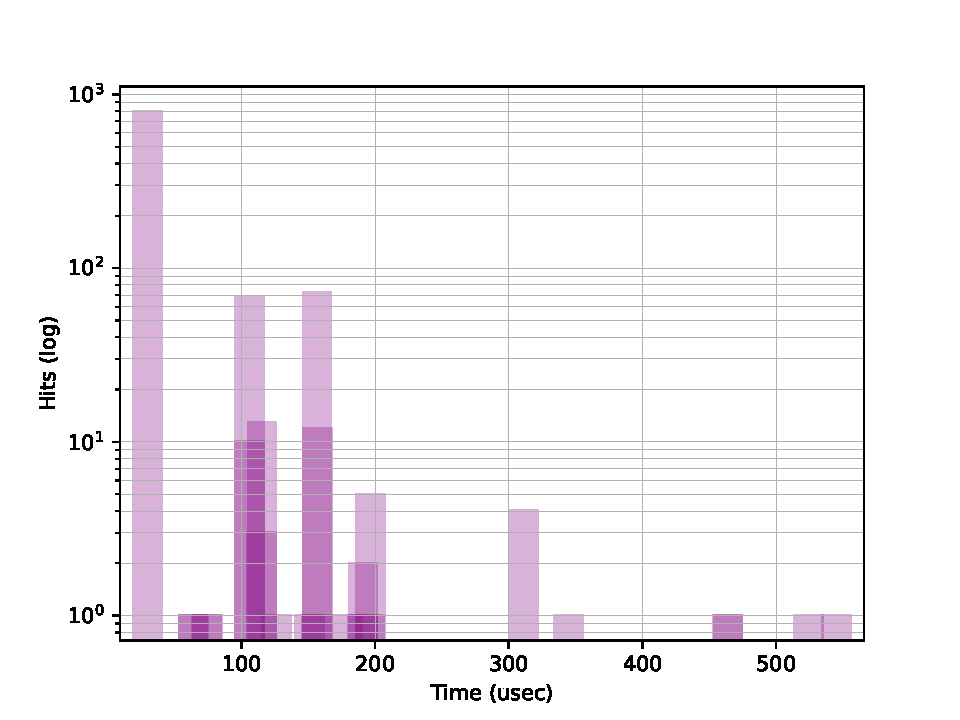
\includegraphics[scale=.4]{assets/reference-value-contiki-z1.pdf}
        \caption{Reference value distribution with Contiki on Z1\label{fig:reference-value-contiki-z1}}
    \end{minipage}\hfill
    \begin{minipage}{.45\textwidth}        
        \centering
        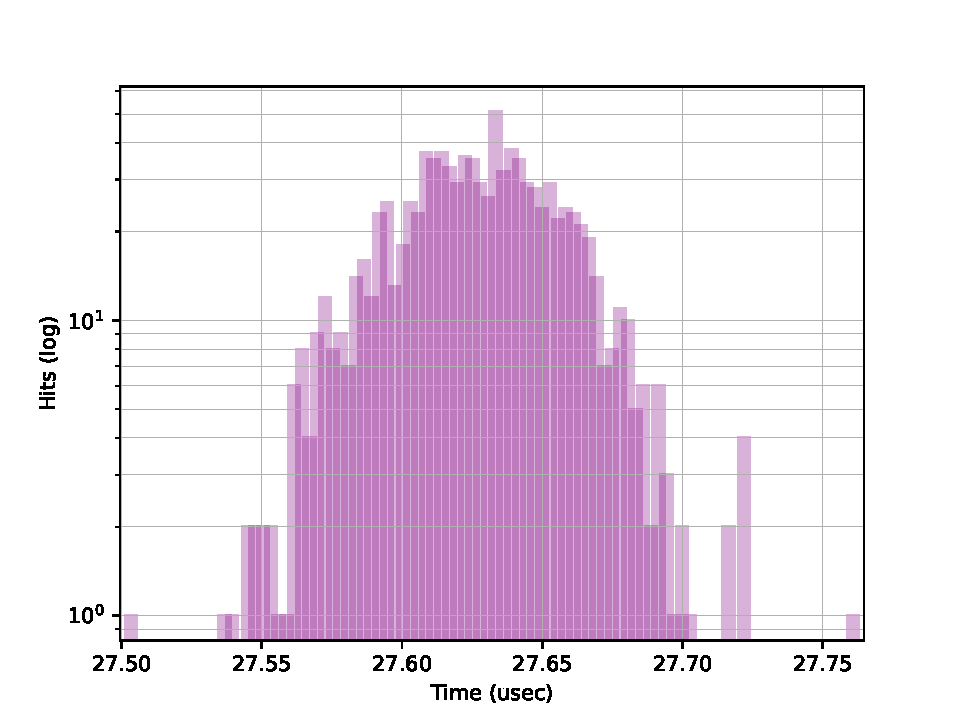
\includegraphics[scale=.4]{assets/reference-value-riot-z1.pdf}
        \caption{Reference value distribution with RIOT OS on Z1\label{fig:reference-value-riot-z1}}
    \end{minipage}
\end{figure}

\subsubsection{Resume}
The table \ref{tab:reference-values-resume} resume our reference values with the two boards, the RE-Mote and the Z1, and the two RTOS, Contiki and RIOT OS.

\begin{table}[!ht]
  \centering
  \begin{tabular}{l|c|c}
                   & Contiki  & RIOT    \\ \hline
  RE-Mote ($\mu$s) & 18.505  & 12.626   \\
  Z1 ($\mu$s)      & 55.077   & 27.699
  \end{tabular}
  \caption{Resume of the reference values}
  \label{tab:reference-values-resume}
  \end{table}

%%%%%% Chap 4 %%%
\chapter{Experiment \label{chap:experiment}}

Before we start to develop our framework, we have contacted and discussed with some of the IoT communities.
Via mailing lists, we communicated with the communities of RIOT OS, Contiki, FreeRTOS, mBed OS and Apache Mynewt.
We also exchanged idea with IoT developers through forums on the web.
Our main concern was to implement a framework that measure the context switching time without altering it.
Indeed, we do not want our framework to slow down the application and adding an overhead.

Unfortunately, the communities and the developpers could not help us.
So, we decided to consider three different approaches.

\section{Integrating the framework in the kernel of the RTOS \label{sec:kernel}}

Our first approach was to implement the framework inside the kernel of the RTOS.
Using this method, we can compute the time it takes for a context switch directly in the scheduler.
In RTOS, when a task goes to the background, the scheduler goes in foreground and resume the next task.
The framework would be able to compute the time between the first and the last call of the scheduler computing this way the context switching time.

\subsection{Motivations}

This approach has some advantages.
First, it make the framework completely hidden for the developer.
This is great because it match one of our criteria for the framework.
The developer could implement its application regardless of the framework operation.
In results, no source code in the user-space should be altered making it possible to use the framework on previously implemented application.
Then, one could use the framework on applications already running in production only by updating the RTOS.

\subsection{Limitations}

Unfortunately, we choose to abandon the approach of integrating the framework inside the kernel of RIOT OS for the following reasons.
First, we were not sure that if we used this methodology we would actually measure the real context switching time.
It is possible that some calls or functions are executed before the scheduler and that the framework will not take them into account.

Finally, the scheduler implementation is strongly platform-dependent meaning that every platform has its own scheduler source code.
It is impossible for us to integrate our framework for each existing platforms.
Some of them are even written in assembly code.
The listing \ref{lst:cpus-riot} shows a truncated list of all the supported platforms by RIOT OS.

\begin{lstlisting}[style=ascii-tree, label={lst:cpus-riot}, caption={Truncated list of platforms supported by RIOT OS}]
cpu/
├── arm7_common
├── atmega1281
├── atmega1284p
(...)
├── stm32l1
└── stm32l4
\end{lstlisting}
\section{Implementing the framework as an extension of the RTOS \label{sec:extension}}

For this second approach, the idea comes from our discussions with the communities.
Instead of building the framework inside the kernel, we would implement the framework as a RTOS extension.
The extension would provide calls that would be used in the user-space of the application.

\subsection{Definition of RTOS extension}

Many RTOS allow developers to create their own extensions that will be used by other developers to enhance and add functionalities to their applications.
In these extensions, we can find libraries that integrates FTP, COAP or even a Shell.
To use those extensions, the developer needs to specify them in the \texttt{Makefile}.
Those libraries are called 'apps' for Contiki and 'modules' for RIOT.

\begin{minipage}{.45\textwidth}
\begin{lstlisting}[style=CStyle, language=make, caption=Example of Makefile using the app \texttt{shell} with Contiki]
CONTIKI_PROJECT = example
all: $(CONTIKI_PROJECT)
CONTIKI = ../contiki

# Using the shell app
APPS += shell 

include $(CONTIKI)/Makefile.include
\end{lstlisting}
\end{minipage}\hfill
\begin{minipage}{.45\textwidth}
\begin{lstlisting}[style=CStyle, language=make, caption=Example of Makefile using the module \texttt{shell} with RIOT]
APPLICATION = example
BOARD ?= native
RIOTBASE ?= $(CURDIR)/../riot

# Using the shell module
USEMODULE += shell 

include $(RIOTBASE)/Makefile.include
\end{lstlisting}
\end{minipage}

\subsection{Framework utilization}

The idea of this second approach is to be able to measure the context switching time without impacting the application.
With this in mind, we will make sure that our framework is called only two times per task iteration.
From these calls, we can deduce the context switching time.
The figure \ref{fig:internal-framework-ping} shows an example with two tasks.
The first task starts at the step A and ends at the step A'.
A context switch occurs between the step A' and the step B, this latter being the start of the second task.
The step B' is the end of the second task.
The idea is to call the framework at each step, A, A', B and B'.
The context switching time is measured between the step A' and B.
The next sections describe the implementation of this framework and what happens when it is used with our simple application.

\begin{figure}[!ht]
  \centering
  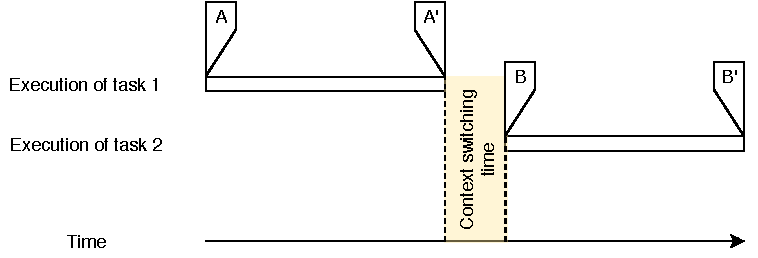
\includegraphics[scale=1]{assets/internal-framework-ping.pdf}
  \caption{\label{fig:internal-framework-ping}Pings to the framework}
\end{figure}

\subsection{Using the framework with our simple application}

To understand the implementation of the framework, we need to understand what happens when our simple application boots 
  and then explain its implementation in the next section.

In the startup of our application, the first task is launched.
It will call the method \texttt{bench\_ping(TASK\_1)} where \texttt{TASK\_1} is the ID of the first task.
At this point, we enter in the framework-space like shown in the figure \ref{fig:extension-activity-framework}.
The framework will check if the received ID from the \texttt{bench\_ping()} call is already stored in its context.
If the received ID match the one stored in the context or if no ID is stored in the context, no context switch occcured and the framework reset its internal timer.
It also store the received ID in its context.
The stored ID is now \texttt{TASK\_1}.
Once the first task ends its iteration and will let the other task runs, it call the same method \texttt{bench\_ping(TASK\_1)} with its ID.
Once again, the framework checks the received ID and no change is detected.
It resets its internal timer.
The stored ID is still \texttt{TASK\_1}.

Now, the second task starts and call the framework with \texttt{bench\_ping(TASK\_2)} where \texttt{TASK\_2} is the ID of the second task.
The framework will detect an ID change by comparing the received ID, \texttt{TASK\_2}, with the stored ID in its context, \texttt{TASK\_1}.
This change means that a context switch occured.
We are between the step A' and B in the figure \ref{fig:internal-framework-ping}.
The framework will measure the context switching time by computing the difference between the actual timer and its internal timer.
The measure is then written on the serial port to be read by an external source like a computer.
The framework resets once again its timer and store the \texttt{TASK\_2} ID in its context.
In this way, we have computed the context switching time between the first and the second task.

\begin{figure}[!ht]
  \centering
  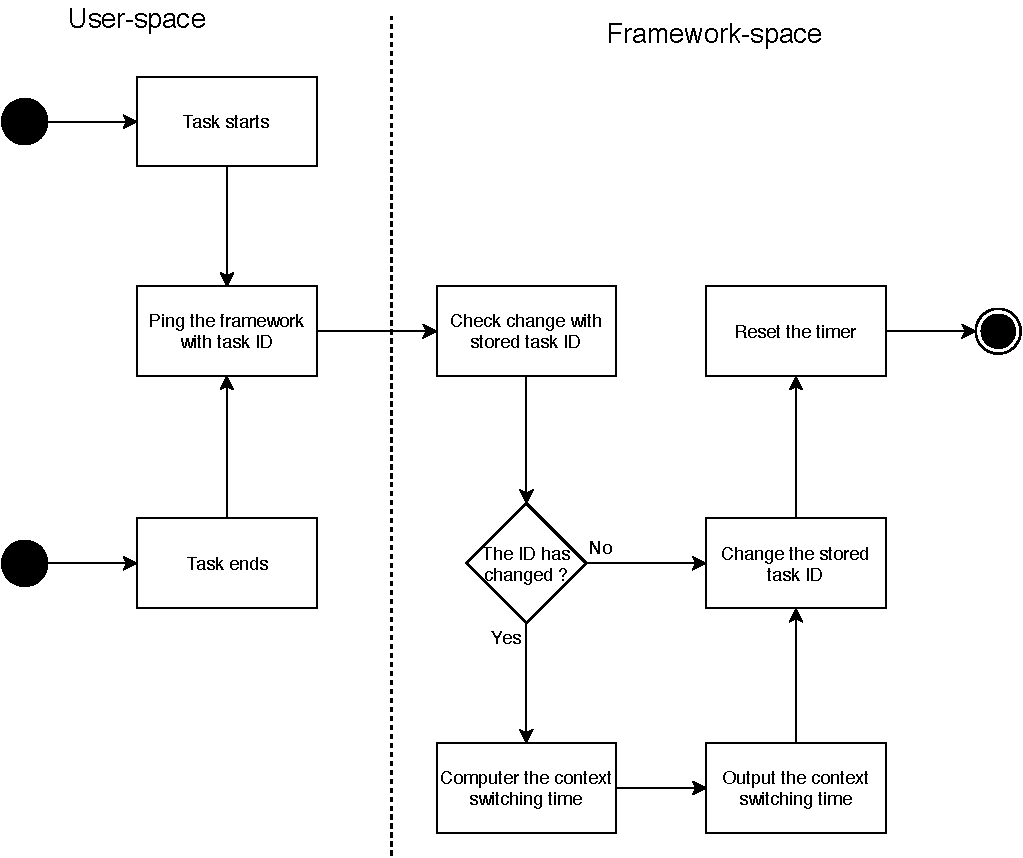
\includegraphics[scale=0.7]{assets/extension-activity-framework.pdf}
  \caption{Activity flow of the framework\label{fig:extension-activity-framework}}
\end{figure}

\subsection{Framework implementation}

\subsubsection{Task source code}
For our simple application source code, we just added the call \texttt{bench\_ping()} at the start and the end of each task.
The listing \ref{lst:bench-task-code} shows how the task source code is impacted in Contiki.

\begin{lstlisting}[float, style=CStyle, label={lst:bench-task-code}, caption={Source code of the application task with \texttt{bench\_ping()} calls}]
PROCESS_THREAD(task, ev, data)
{
    PROCESS_BEGIN();

    while (1)
    {
      bench_ping(TASK_ID); // Ping the framework
      // Wait for 1ms
      clock_delay_usec(1000);
      bench_ping(TASK_ID); // Ping the framework
      PROCESS_PAUSE();
    }

    PROCESS_END();
}
\end{lstlisting}

\subsubsection{Framework source code}

For the framework context, we store the received ID in the \texttt{new\_id} variable 
  and then use the \texttt{previous\_id} variable to check if a context switch occured.
The \texttt{current\_time} variable is the interval timer.
The code of the framework context is shown in the listing \ref{lst:context-code}.

\begin{lstlisting}[style=CStyle, float, label={lst:context-code}, caption={Framework context implementation}]
struct BContext {
  uint32_t previous_id;
  uint32_t new_id;
  clock_time_t current_time;
} bench_context;
\end{lstlisting}

The \texttt{bench\_ping()} method will just saved the received ID in the \texttt{new\_id} variable 
  and then check if a change is detected like shown in the listing \ref{lst:bench-ping-code}.

\begin{lstlisting}[style=CStyle, float, label={lst:bench-ping-code}, caption={\texttt{bench\_ping()} implementation}]
void bench_ping(uint32_t id)
{
  bench_context.new_id = id;
  if (!check_change())
  {
    bench_context.current_time = RTIMER_NOW();
  }
}
\end{lstlisting}

When a change is detected, the framework will compute the context switching time 
  by retrieving the current time and computing its difference with \texttt{current\_time} variable.
The time is computed in ticks for a better precision.
To retrieve the time in ticks, we used \texttt{RTIMER\_NOW()} in Contiki and \texttt{xtimer\_now().ticks32} in RIOT.
The internal timer is then reset just before writting the measure into the serial port.
Then the measure is written to the serial port using the \texttt{printf()} call.
The code of this measurement is shown in the listing \ref{lst:measurement-code}.

\begin{lstlisting}[style=CStyle, float, label={lst:measurement-code}, caption={Source code of the benchmarking framework implemented in Contiki}]
// Compute the difference
clock_time_t previous = bench_context.current_time;
clock_time_t current = RTIMER_NOW();
clock_time_t result = current - previous;

// Keep the previous id for log
uint32_t previous_id = bench_context.previous_id;
// Change previous_id to new_id
bench_context.previous_id = bench_context.new_id;

bench_context.current_time = RTIMER_NOW(); // Ticks

printf("[BENCH_CONTEXT_SWITCHING] %lu %lu %lu\n", previous_id, bench_context.new_id, result);
\end{lstlisting}

All the source codes can be found in the \href{https://github.com/bench-os/bench-os}{Github repository}.
\section{Using external devices \label{sec:external}}

Our third and last approach was to use external devices to compute the context switching time.
In this way, all the heavy computational processes are done outside of the board but in a computer, for example.

\subsection{Choice of the external device}

Our first idea was to implement it with Python3.7 on a desktop computer.
Using the UART protocol over USB, the board sends a single byte containing the thread ID that is read by a Python script on the computer.

The motivations for using this alternative are:
\begin{itemize}
  \item Sending one byte of data over USB with UART have a smaller impact than computing the context switching time locally on the board;
  \item Heavy computational tasks of the framework are done on the computer and not on the board;
  \item Using Python3.7, we can achieve a time precision at the nanosecond.
\end{itemize}

However, after discussing with the embedded community, we abandonned this idea for the following reasons.
There is buffering happening on the USB-serial chip on the board, on the PC's USB hardware, in the PC USB-serial driver and also in the desktop operating systems.
Those buffering will add delay in our measurements.
Context switchs will occur on the desktop computer that will invalidate any timing value.

Instead, we decided to use a device called the Pocket Science Lab to perform our experiment.

\begin{figure}[!ht]
  \centering
  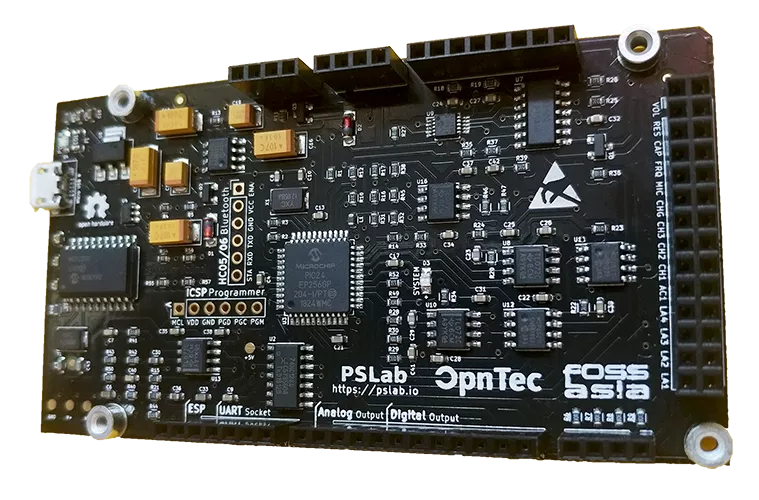
\includegraphics[scale=0.25]{assets/pslab.png}
  \caption{\label{fig:pslab}Pocket Science Lab device from \href{https://pslab.io}{PSLab.io}}
\end{figure}

The Pocket Science Lab device from \href{https://pslab.io}{PSLab.io} comes with a built-in 4-Channel up to 2MSPS oscilloscope, multimeter, 4-Channel, 4 MHz logic analyser, and other digital instruments.
Using the Python librairy \href{https://github.com/fossasia/pslab-python}{pslab-python}, we can communicate with the board and experiment with it.
With a device like the PSLab, we can left the benchmarked board that contains our simple application untouched in terms of heavy computations.

\subsection{Roles of the devices}

With the benchmarked board, the PSLab and the computer, we have three devices that we use to compute the context switching time.
The figure \ref{fig:external-benchmarking-framework-schema} shows the connections between the different devices.
To make some clarity, we have defined a specific role to each device.

\subsubsection{The benchmarked board}
The benchmarked board runs the RTOS of our choice with our benchmarking framework and our simple application.
It communicate with our computer through UART and with the PSLab using a single GPIO.
Its role is to simply run the application and change the state of the GPIO depending on the tasks status.

\subsubsection{The computer}
The computer is the brain of the benchmarking framework.
It is responsible of communicating with both the benchmarked board and the PSLab through the UART protocol.
It is its responsability to coordinate the benchmarked board and the PSLab in order to retrieve the context switching time.
The computer is also the place where all the data are accumulated.

\subsubsection{The PSLab}
Connected with a single GPIO to the benchmarked board, the PSLab watch for any context switch.
It measure the context switching time using its logical analyser.
The board receives its instruction and send the measures through UART with our computer.

\begin{figure}[!ht]
  \centering
  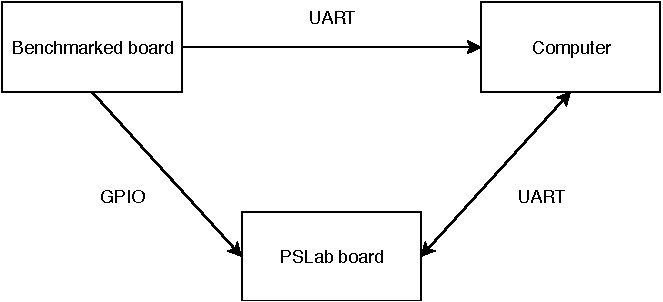
\includegraphics[scale=1]{assets/external-benchmarking-framework-schema.pdf}
  \caption{\label{fig:external-benchmarking-framework-schema}Interaction schema of the devices used in the framework}
\end{figure}

\subsection{Usage of the Pocket Science Lab}

The PSLab will monitor a single GPIO and measure the context switching time from it.
The figure \ref{fig:external-framework-context-switching-time-measurement} shows the steps in the measurement with the PSLab.
Each task will set the GPIO up at the start of its execution and then reset the GPIO once it ended.
In our example, the task 1 set up the GPIO at the step A and the GPIO is in high position at step A'.
Once the task 1 is finished, it reset the GPIO at the step B that will be in position at step B'.
The same process occurs for the task 2.
The task 2 set up the GPIO at step C.
The GPIO is in high position at step C'.
Finally, the task 2 reset the GPIO at the end of its execution at step D and the GPIO will be in position low at step D'.
From our measurements made with the reference value, we know that the rising time of the GPIO is around 10 nanoseconds so it can be omitted.

\begin{figure}[!ht]
  \centering
  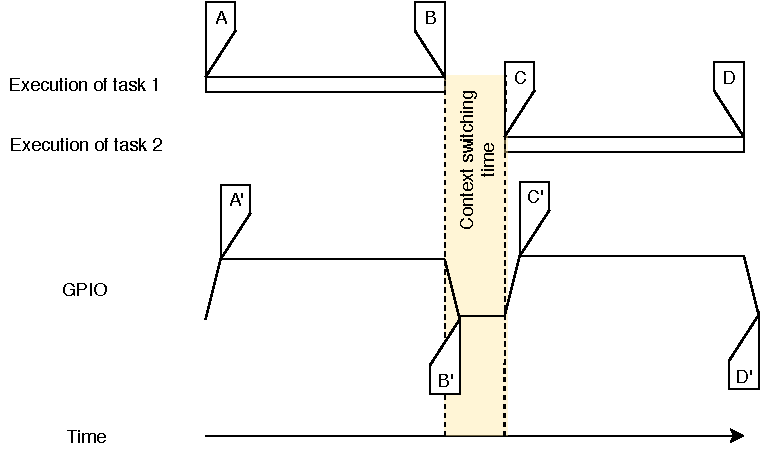
\includegraphics[scale=1]{assets/external-framework-context-switching-time-measurement.pdf}
  \caption{\label{fig:external-framework-context-switching-time-measurement}Measurement of the context switching time with a single GPIO}
\end{figure}

\subsection{Using the framework with our simple application}

To understand the framework implementation, it is important to understand what happens when our simple application boots.
But both from the point of view of the benchmarked board and from the point of view of the PSLab and the computer.

\subsubsection{Point of view of the benchmarked board}
When the application boots, it will initialize the framework.
An initializiation is required to use the GPIO.
Once the initializiation is done, the first task starts.
It will call \texttt{bench\_on()} from the framework.
In the framework-space, \texttt{bench\_on()} will have for effect to set the GPIO up.
When the task is done, it will call \texttt{bench\_off()} that will reset the GPIO.
The second task goes in the foreground and will also call \texttt{bench\_on()} and, latter, \texttt{bench\_off()}.

\subsubsection{Point of view of the PSLab and the computer}
The PSLab will listen for an interval between a falling and a rising edge.
In the figure \ref{fig:external-framework-context-switching-time-measurement}, this interval happens between the step B' and C'.
For reminder, the rising time can be omitted.
Once the PSLab detect an interval, it compute its time.
This interval time is the context switching time.
This measure is send to the computer that will store it.

\subsection{Framework implementation}

The interaction between the benchmarked board and the PSLab is done through a GPIO that is controlled by the benchmarked board.
The code in the benchmarked board is quite straightforward.
First, our simple application need initialize the framework and start its tasks.
Then, we need to add \texttt{bench\_on()} and \texttt{bench\_off()} respectively at the start and at the end of the two tasks.
The code of the updated application is shown in the listing \ref{lst:external-app-code}.

\begin{lstlisting}[style=CStyle, float, caption={Source code of the simple application in Contiki}, label={lst:external-app-code}]
#include "contiki.h"
#include "sys/clock.h"
#include "bench-context-switching.h"

#include <stdio.h>

PROCESS(init_task, "Init task");
PROCESS(task_1, "First task");
PROCESS(task_2, "Second task");
AUTOSTART_PROCESSES(&init_task);

PROCESS_THREAD(init_task, ev, data)
{
    PROCESS_BEGIN();

    bench_init();

    process_start(&task_1, NULL);
    process_start(&task_2, NULL);

    PROCESS_END();
}

PROCESS_THREAD(task_1, ev, data)
{
    PROCESS_BEGIN();

    while (1)
    {
        bench_on();
        clock_delay_usec(1000);
        bench_off();
        PROCESS_PAUSE();
    }

    PROCESS_END();
}

// ...
// task_2 is identical to task_1
\end{lstlisting}

During the initializiation, the framework will setup the GPIO as an output port. The listing \ref{lst:external-init-code} shows this process.
The \texttt{bench\_on()} and \texttt{bench\_off()} will just set or reset the GPIO like shown in the listing \ref{lst:external-on-off-code}.

\begin{lstlisting}[style=CStyle, caption={Initializiation of the framework in Contiki}, label={lst:external-init-code}]
void bench_init()
{
    GPIO_SOFTWARE_CONTROL(GPIO_PORT_TO_BASE(GPIO_C_NUM), GPIO_PIN_MASK(2));
    GPIO_SET_OUTPUT(GPIO_PORT_TO_BASE(GPIO_C_NUM), GPIO_PIN_MASK(2));
}
\end{lstlisting}

\begin{lstlisting}[style=CStyle, caption={\texttt{bench\_on()} and \texttt{bench\_off()} implementation in Contiki}, label={lst:external-on-off-code}]
void bench_on(uint32_t pid)
{
    GPIO_SET_PIN(GPIO_PORT_TO_BASE(GPIO_C_NUM), GPIO_PIN_MASK(2));
}

void bench_off()
{
    GPIO_CLR_PIN(GPIO_PORT_TO_BASE(GPIO_C_NUM), GPIO_PIN_MASK(2));
}
\end{lstlisting}

Finally, from the computer, we need to retrieve and store the interval measurement from the PSLab.
To do so, we use a Python script shown in listing \ref{lst:python-pslab} that connect to the PSLab and retrieve the context switching time between a falling and a rising edge.

\begin{lstlisting}[style=CStyle, language=python, caption={Python script to communicate with the PSLab and retrieve the interval measurement}, label={lst:python-pslab}]
from PSL import sciencelab
I = sciencelab.connect()

VALUES = []

while True:
    CS_TIME = I.MeasureInterval('ID1', 'ID1', 'falling', 'rising')
    VALUES.append(CS_TIME)
\end{lstlisting}


% In order to implement this third approach, we need to update our simple task, create our framework in Contiki as an app and creating a Python script that will run on the computer and communicate with both the benchmarked board and the PSLab.

% \subsubsection{Protocol}

% We first need to define some sort of protocol to communicate between our three devices.
% The figure \ref{fig:external-protocol} shows the interactions between every device.

% \begin{figure}[!ht]
%   \centering
%   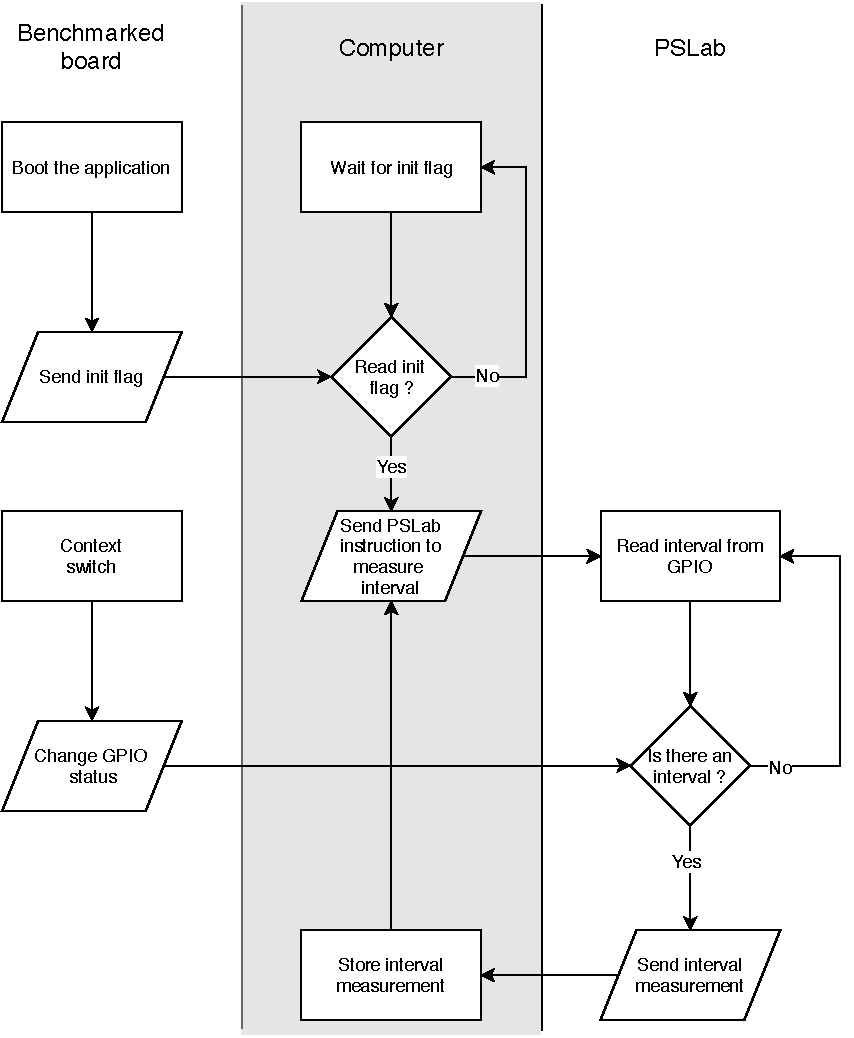
\includegraphics[scale=0.7]{assets/external-protocol.pdf}
%   \caption{\label{fig:external-protocol}Schema of the protocol used between the devices}
% \end{figure}

% The first step is to start the Python script on the computer. It will read all the messages send by the board on the UART port.
% When the benchmarked board boots, it will send an init flag to the computer once its GPIO is setup and it is ready to transmit information through the GPIO.
% Once the computer read the init flag, it will send to the PSLab the instruction to read a time interval between a falling and a rising edge like shown in the figure \ref{fig:external-framework-context-switching-time-measurement}.
% Once a task is done in the benchmarked board, it will reset the GPIO that will trigger the PSLab measurement.
% This measurment is send to the computer and the computer will save the value.
% The computer will then send the instruction to the PSLab again and wait for a new measurement.

% \subsubsection{Python script}

% The Python script that run on the computer is the coordinator of the framework.
% The first thing it does is to read the UART port and wait for the init flag from the benchmarked board.
% Once it read the flag, it send the same flag to the benchmarked board and enter in an infinite loop where it will fetch the interval measurements from the PSLab using the \texttt{MeasureInterval()} call.
% Every time a value is received from the PSLab, it is stored in an array.
% The source code of the script is in the listing \ref{lst:pslab-script-code}.

% \begin{lstlisting}[style=CStyle, float, language=python, label={lst:pslab-script-code}, caption={Python script source code}]
% """
% This script retrieves the context switching time between two tasks.
% """
% import serial
% from PSL import sciencelab

% BENCH_CONTEXT_SWITCHING_FLAG = '[BENCH_CONTEXT_SWITCHING]' 
% SER = serial.Serial('/dev/ttyUSB0', 115200)

% I = sciencelab.connect()
% VALUES = []

% ready = False
% while not ready:
%     try:
%         line = str(SER.readline(), 'utf-8')
%         if BENCH_CONTEXT_SWITCHING_FLAG in line:
%             if "Ready" in line:
%                 SER.write(bytes("{} Ready\n".format(BENCH_CONTEXT_SWITCHING_FLAG), 'utf-8'))
%                 ready = True
%     except:
%         pass

% while True:
%     CS_TIME = I.MeasureInterval('ID1', 'ID1', 'falling', 'rising')
%     VALUES.append(CS_TIME)
% \end{lstlisting}

% \subsubsection{Contiki extension}
% The extension in Contiki define four functions used by the application.
% First the \texttt{bench\_init()} function that will setup the GPIO and send the init flag through the serial port.
% Then, the \texttt{bench\_chech\_data(char*)} that will check if the received message from the computer is the init flag.
% Finally, the \texttt{bench\_on()} and \texttt{bench\_off()} functions that will respectively set up and reset the GPIO.
% The source code of the extesion in Contiki can be found in the listing \ref{lst:external-framework-code}.


% \begin{lstlisting}[style=CStyle, float, label={lst:external-framework-code}, caption={Source code of the extesion in Contiki}]
% #include "bench-context-switching.h"

% void bench_init()
% {
%     // Setup the GPIO
%     GPIO_SOFTWARE_CONTROL(GPIO_PORT_TO_BASE(GPIO_C_NUM), GPIO_PIN_MASK(2));
%     GPIO_SET_OUTPUT(GPIO_PORT_TO_BASE(GPIO_C_NUM), GPIO_PIN_MASK(2));
%     // Start the benchmark
%     printf("%s Ready\n", BENCH_CONTEXT_SWITCHING_FLAG);
% }

% int bench_check_data(char* data)
% {
%     int size = strlen(BENCH_CONTEXT_SWITCHING_FLAG) + strlen(" Ready\n") + 1;
%     char str[size];
%     sprintf(str, "%s Ready\n", BENCH_CONTEXT_SWITCHING_FLAG);
%     return strcmp(str, data);
% };

% void bench_on()
% {
%     // Set the GPIO up
%     GPIO_SET_PIN(GPIO_PORT_TO_BASE(GPIO_C_NUM), GPIO_PIN_MASK(2));
% }

% void bench_off()
% {
%     // Reset the GPIO
%     GPIO_CLR_PIN(GPIO_PORT_TO_BASE(GPIO_C_NUM), GPIO_PIN_MASK(2));
% }
% \end{lstlisting}

% \subsubsection{Simple task}
% The simple task in Contiki will first init the benchmarking framework and wait for the init flag received from the computer.
% Once it receives a confirmation from the computer, it will start the tasks with the \texttt{process\_start()} call.
% Each task will use the \texttt{bench\_on()} and \texttt{bench\_off()} calls from the benchmarking framework.
% Those calls will cause the GPIO to be in high position when a task is in the foreground and be in low position when no task is running.

% \begin{lstlisting}[style=CStyle, float, label={lst:external-task-code}, caption={Source code of a task using the benchmarking framework}]
% #include "contiki.h"
% #include "sys/clock.h"
% #include "bench-context-switching.h"
% #include <stdio.h>

% PROCESS(init_task, "Init task");
% PROCESS(task, "Task");
% AUTOSTART_PROCESSES(&init_task);

% int bench_context_switching_ready = 0;

% PROCESS_THREAD(init_task, ev, data)
% {
%     PROCESS_BEGIN();

%     bench_init();

%     while (!bench_context_switching_ready)
%     {
%         PROCESS_YIELD();
%         if(ev == serial_line_event_message) {
%             printf("received line: %s\n", (char *)data);
%             bench_context_switching_ready = bench_check_data((char *)data);
%         }
%     }

%     process_start(&task, NULL);

%     PROCESS_END();
% }

% PROCESS_THREAD(task, ev, data)
% {
%     PROCESS_BEGIN();

%     while (1)
%     {
%         bench_off();
%         PROCESS_PAUSE();
%         bench_on();
%         clock_delay_usec(1000);
%     }

%     PROCESS_END();
% }
% \end{lstlisting}


%%%%%% Chap 5 %%%
\chapter{Results and framework measurements \label{chap:results}}

This chapter give the all the measurements gathered during our experiments.
Those results are given without any comment.
Each presented plot have a logarithmic y-axis.
The chapter \ref{chap:discuss} discusses the results and compare the two approaches.
The first section gives mesures of the approaches impact.
The second section gives the obtained measurements with the two approaches.

For each approach, 1000 measurements were made on the two RTOS, Contiki and RIOT, and on the two boards, the RE-Mote and the Z1 boards for a total of 4000 measurements. From these measurements, the statistics used were the mean, the minimum and the maximum.

\section{Overhead}

One of our first concerns was to implement a framework that does not impact to our simple application.
The benchmarking framework shoul be hidden for the developer.
Enabling the framework should not altering the good use of the application.

To mesure the impact of our approaches, we used the same setup than with our reference value and retrieve 1000 measurements of the context switching time.
We compared those measurements with our reference value and compute the overhead of our framework.
The oscilloscope measurements are shown in the figure \ref{fig:overhead-reference-value-contiki-z1}.

\subsection{Extension approach overhead}

The extension approach have a large overhead of more than 2ms for with RE-Mote board and more than 3ms with the Z1 board on both Contiki and RIOT.
On the figure \ref{fig:overhead-extension-contiki-z1}, we can see the overhead of the first approach with the measurements made by the oscilloscope.
We discuss later why our extension approach add such a latency in the section \ref{sec:overhead}.

\subsection{Devices approach overhead}

The devices approach, in the other hand, have a small overhead of less than $3\mu s$ with either the RE-Mote or the Z1 boards on both Contiki and RIOT.
On the figure \ref{fig:overhead-devices-contiki-z1}, we can see the overhead of the devices approach.
The devices approach add a much more smaller overhead to our simple application than the extension approach.
This difference between the overhead of the two approaches is discussed in the section \ref{sec:overhead}.

\begin{figure}[!ht]
        \centering
        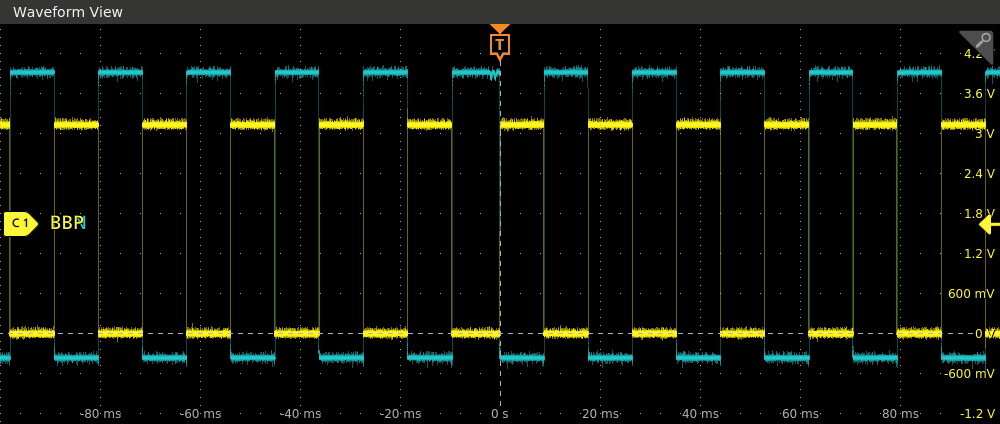
\includegraphics[scale=.4]{assets/reference-value-overhead-contiki-z1.png}
        \caption{overhead reference measured by the oscilloscope\label{fig:overhead-reference-value-contiki-z1}}

        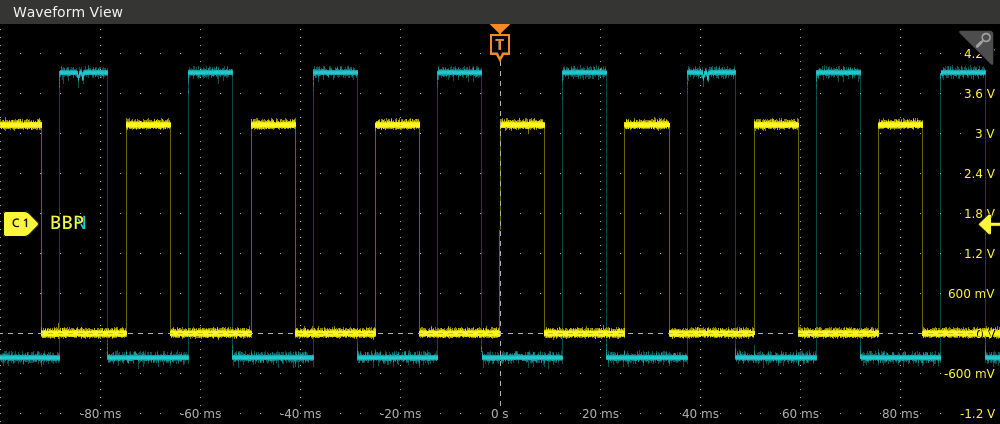
\includegraphics[scale=.4]{assets/extension-framework-overhead-contiki-z1.png}
        \caption{extension approach overhead measured by the oscilloscope\label{fig:overhead-extension-contiki-z1}}

        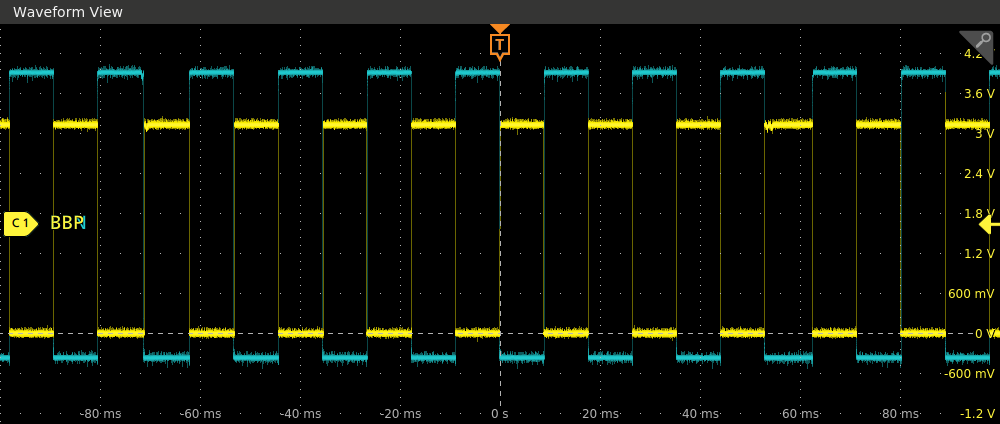
\includegraphics[scale=.4]{assets/devices-framework-overhead-contiki-z1.png}
        \caption{devices approach overhead measured by the oscilloscope\label{fig:overhead-devices-contiki-z1}}
\end{figure}

\section{Framework measurements}

We describe in this section the results gathered with the extension approach described in the section \ref{sec:extension} and with the devices approach described in the section \ref{sec:external}.
For recall, the first approach is to implement the framework as a RTOS module used in the user space and that will compute internally the context switching time.
The second approach is to measure the context switching time using an external board, the PSLab.

In the same way as with the reference value, the results are divided by boards.
The measurements made with the RE-Mote boards are first given, then the one made with Z1 board.
The Contiki measurements are displayed side-by-side with the RIOT one for more clarity.

\subsection{Extension approach measurements}

\subsubsection{RE-Mote board measurements}
With Contiki, the framework outputs measurements with an average of 31.6162 $\mu$s.
With 0$\mu$s as the minimum value and 457.7636 $\mu$s as the maximum value, the measurements have a large distribution.
We have a difference of 13.1112 $\mu$s between the measured context switching time and the real one measured with the oscilloscope.

With RIOT, the framework outputs a constant context switching time of 17 $\mu$s.
All 1000 measurements were equal to 17 $\mu$s.
Thus, the difference with the real context switching time is 4.374 $\mu$s.

Both measurements were above the real context switching time given by the reference value.
The table \ref{tab:extension-framework-remote} shows the measurement for Contiki and RIOT for the RE-Mote board.

\begin{table}[!ht]
  \centering
  \begin{tabular}{l|c|c}
                & Contiki  & RIOT \\ \hline
  Mean ($\mu$s) & 31.6162  & 17      \\
  Min  ($\mu$s) & 0        & 17      \\
  Max  ($\mu$s) & 457.7636 & 17     
  \end{tabular}
  \caption{extension approach measurements for Contiki and RIOT on the RE-Mote board}
  \label{tab:extension-framework-remote}
  \end{table}

\subsubsection{Z1 board measurements}
On the Class-1 Z1 board, the framework gave an average context switching time of 90.5761 $\mu$s with Contiki.
Once again, on Contiki, our values were largely distributed between 30.5175 $\mu$s and 976.5625 $\mu$s.
The average context switching time measured is 35.4991 $\mu$s above the real context switching time.

With RIOT, most of the values were equal to 40 $\mu$s with an average of 40.252 $\mu$s.
This put the measurements 12.553 $\mu$s above the real context switching time.

The table \ref{tab:extension-framework-z1} shows the measurement for Contiki and RIOT for the Z1 board.

\begin{table}[!ht]
  \centering
  \begin{tabular}{l|c|c}
                & Contiki  & RIOT \\ \hline
  Mean ($\mu$s) & 90.5761  & 40.252      \\
  Min  ($\mu$s) & 30.5175  & 40      \\
  Max  ($\mu$s) & 976.5625 & 41     
  \end{tabular}
  \caption{extension approach measurements for Contiki and RIOT on the Z1 board}
  \label{tab:extension-framework-z1}
  \end{table}

\subsection{Devices approach measurement}

\subsubsection{RE-Mote board measurements}
On the RE-Mote board, the devices approach outputs an average context switching time of 19.0329 $\mu$s on Contiki.
This measurement differs from the real context switching time by only 2.85$\%$.
They are 0.5279 $\mu$s above the reference measurements.
The majority of the values were around 14 $\mu$s but some of them were above 40 $\mu$s.
The figure \ref{fig:devices-framework-contiki-remote} show the distribution of the measurements made with Contiki.

\begin{figure}[!ht]
      \centering
      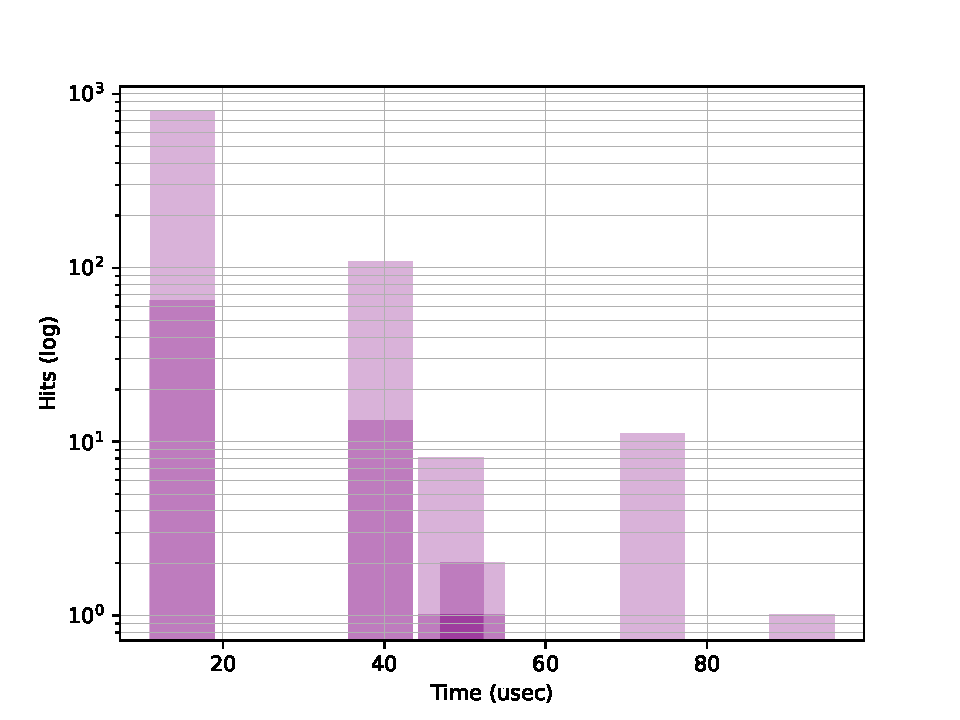
\includegraphics[scale=.7]{assets/devices-framework-contiki-remote.pdf}
      \caption{devices approach measurements distribution with Contiki on the RE-Mote board\label{fig:devices-framework-contiki-remote}}
\end{figure}

With RIOT, the average context switching was 12.9832 $\mu$s.
For RIOT, the measurement were either around 12.95 $\mu$s or around 13 $\mu$s.
The figure \ref{fig:devices-framework-riot-remote} shows this disparity.
The measured context switching time is above the real context switching time by 0.3572 $\mu$s.
This represents an offset of $2.82\%$ from the reference measurements.

\begin{figure}[!ht]
      \centering
      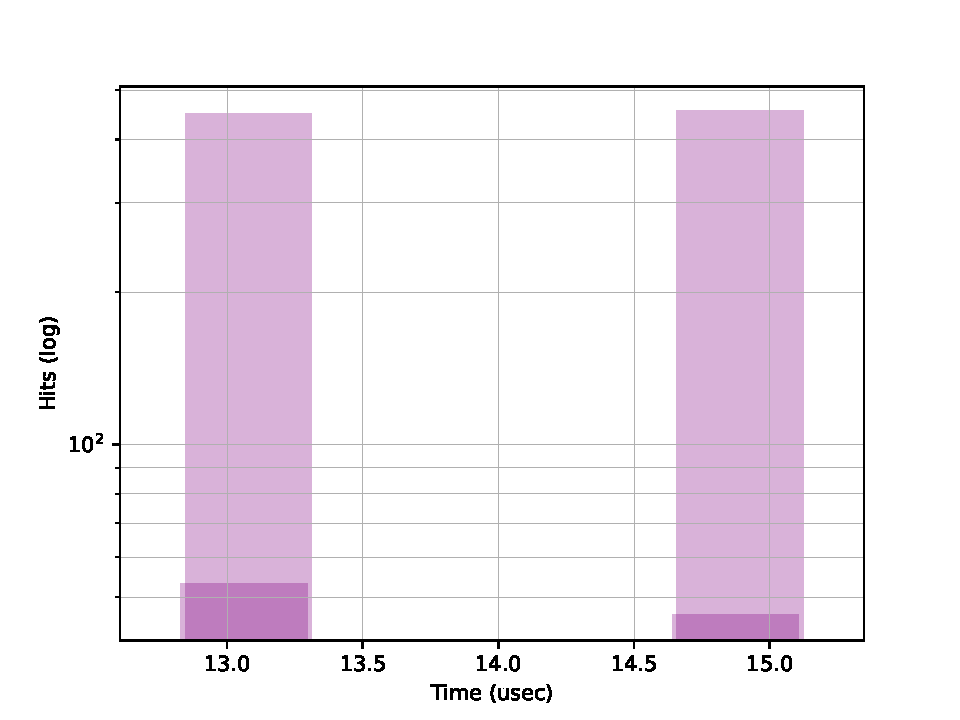
\includegraphics[scale=.7]{assets/devices-framework-riot-remote.pdf}
      \caption{devices approach measurements distribution with RIOT on the RE-Mote board\label{fig:devices-framework-riot-remote}}
\end{figure}

The table \ref{tab:devices-framework-remote} shows the measurement for Contiki and RIOT for the RE-Mote board.

\begin{table}[!ht]
  \centering
  \begin{tabular}{l|c|c}
                & Contiki  & RIOT \\ \hline
  Mean ($\mu$s) & 19.0329  & 12.9823 \\
  Min  ($\mu$s) & 14.9375  & 12.9375 \\
  Max  ($\mu$s) & 91.75    & 13.0156
  \end{tabular}
  \caption{devices framework measurements for Contiki and RIOT on the RE-Mote board}
  \label{tab:devices-framework-remote}
  \end{table}

\subsubsection{Z1 board measurements}
With the second approach, on the Z1 board, the framwork found an average context switching time of 54.99 $\mu$s with Contiki.
The framework measurements were $0.15\%$ off from the real measurements by being 0.087 $\mu$s below them.
However, with Contiki the measured values are more scattered like shown in the figure \ref{fig:devices-framework-contiki-z1}.
The minimum measured context switching time is 32.5625 $\mu$s and the maximum one is 314.5 $\mu$s.

\begin{figure}[!ht]
      \centering
      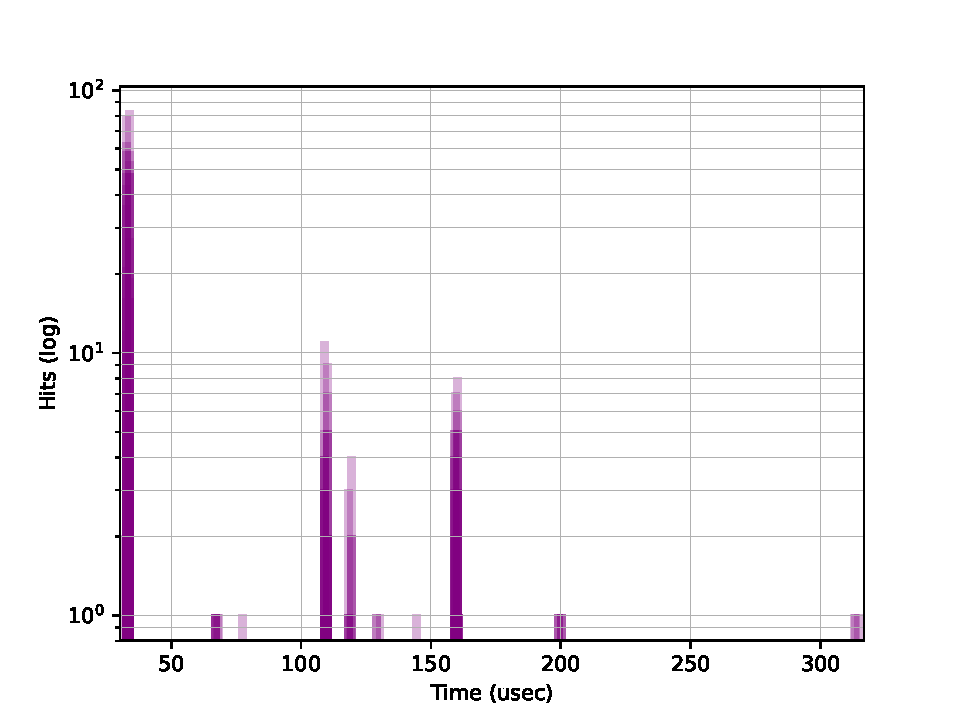
\includegraphics[scale=.7]{assets/devices-framework-contiki-z1.pdf}
      \caption{devices approach measurements distribution with Contiki on the Z1 board\label{fig:devices-framework-contiki-z1}}
\end{figure}

With RIOT, the framework outputted an average context switching time of 30.6971 $\mu$s.
The difference with the real context switching time is 2.9981 $\mu$s making the framework measurements more than $10\%$ above the reference measurements.
On the other hand, the framework measurements gave the same distribution as the one found with the oscilloscope in the section \ref{sec:ref-measurements} with the figure \ref{fig:reference-value-riot-z1}.
The measured measurements distribution is shown in the figure \ref{fig:devices-framework-riot-z1}.

\begin{figure}[!ht]
      \centering
      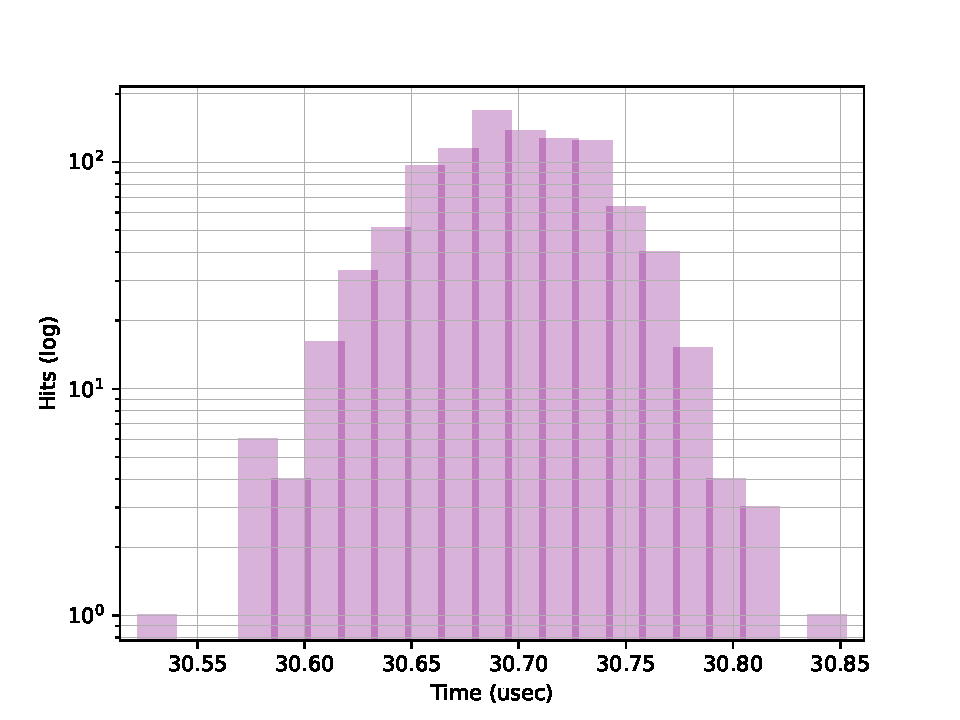
\includegraphics[scale=.7]{assets/devices-framework-riot-z1.pdf}
      \caption{devices approach measurements distribution with RIOT on the Z1 board\label{fig:devices-framework-riot-z1}}
\end{figure}

The table \ref{tab:devices-framework-z1} shows the measurement for both Contiki and RIOT on the Z1 board.

\begin{table}[!ht]
  \centering
  \begin{tabular}{l|c|c}
                & Contiki  & RIOT OS \\ \hline
  Mean ($\mu$s) & 54.99    & 30.6971 \\
  Min  ($\mu$s) & 32.5625  & 30.5312 \\
  Max  ($\mu$s) & 314.5    & 30.8437
  \end{tabular}
  \caption{devices framework measurements for Contiki and RIOT on the Z1 board}
  \label{tab:devices-framework-z1}
  \end{table}

\subsection{Resume}
To give more clarity to the results, the following tables give the average context switching time measured with the two approaches.
The table \ref{tab:framework-measurements-resume-remote} gives the measurements made on the RE-Mote board.
The table \ref{tab:framework-measurements-resume-z1} gives the measurements made on the Z1 board.
The difference between the measured context switching time and the real context switching time measured with the oscilloscope is written between parenthesis.

\begin{table}[!ht]
  \centering
  \begin{tabular}{l|c|c}
                      & Contiki           & RIOT             \\ \hline
  Extension approach ($\mu s$) & 31.6162 (13.1112) & 17 (4.374)       \\
  Devices approach ($\mu s$)   & 19.0329 (0.5279)  & 12.9832 (0.3572)
  \end{tabular}
  \caption{Framework measurements resume on the RE-Mote board}
  \label{tab:framework-measurements-resume-remote}
  \end{table}

\begin{table}[!ht]
  \centering
  \begin{tabular}{l|c|c}
                      & Contiki           & RIOT             \\ \hline
  Extension framework ($\mu s$) & 90.5761 (35.4991) & 40.252 (12.553)       \\
  Devices framework ($\mu s$)   & 54.99 (-0.087)  & 30.6971 (2.9981)
  \end{tabular}
  \caption{Framework measurements resume on the Z1 board}
  \label{tab:framework-measurements-resume-z1}
  \end{table}


%%%%%% Chap 6 %%%
\chapter{Discussion and comparison of the approaches}

During our experiments, we have tried to measure the context switching time of a RTOS with two different approaches.
In this chapter, we discuss and interprate the obtained results described in the previous chapter \ref{chap:results}.
From those results, we describe four observations that we have made in the following sections.

\section{Extension framework overhead issue\label{sec:overhead}}

With our first approach, the framework adds to our simple application a large overhead of more than 2ms for every context switch.
This is an issue for our benchmarking framework as it should have a minimal impact on our application.
With such an overhead, the RTOS loose its real-time capabilities.
It become impossible for the RTOS to react in time to interrupts.

\subsection{Causes}

Sending measurements throught the serial port create this latency.
Indeed, the framework send a string that contains the measured value in order for the computer to read it.
For example, the listing \ref{lst:print-string} shows how the framework write the measurements on the serial port with the method \texttt{printf()} with Contiki

\begin{lstlisting}[style=CStyle, float, label={lst:print-string}, caption={writting the measurements to the serial port with Contiki}]
  printf("[BENCH_CONTEXT_SWITCHING] %lu %lu %lu\n", previous_id, bench_context.new_id, result);
\end{lstlisting}

The string \texttt{[BENCH\_CONTEXT\_SWITCHING]} is a flag used to differenciate framework outputs from the application outupts.
However, printing out at least 32 characters for every context switch on the serial port even at 250 kbit/s took 1.2ms.

\subsection{Solutions and improvements}

To improve the extension approach, one optimization could be to reduce the number of bits send through the serial port.
By sending compressed data and using only a small number of bytes, it could be possible to reduce the overhead.
But even with 8 bits for the flag an 32 bits for the context switching time, 40 bits would take up to $160\mu s$ to be transmitted.

In addition to compress the data, another solution would be to use a cache storing the measurements.
This cache would be flushed and the values written on the serial port at appropriate times.
Either when the cache is full or with a framework method that would allow the developer to choose when to flush the cache.
This way, the overhead occurs not at each context switch but only at appropriate time.

\subsection{Overhead of the devices framework}

In the other hand, the devices approache have a small impact on the system with an overhead of less than $3\mu s$ per context switch.
Even if it is a small overhead, it is however present.
Our hypothesis on this overhead is that the framework calls, \texttt{bench\_on()} and \texttt{bench\_off()} have an impact on the system.
However, there is no fact supporting this conclusion.
\section{Assessment of the different approaches}

Based on our reference measurements from the section \ref{sec:reference}, we can assess the performances of our two different approaches.
To determine which approach perform the best, the difference between the measured context switching time and the real one is used.
Moreover, comparing the distributions of the measurements can refine the analysis.

\subsection{Extension approach performance}

For our extension approach, we can say that it performs poorly.
For example, on Contiki with the RE-Mote board, the expected context switching time is 18.505 $\mu$s but our framework measured a context switching time of 31.6162 $\mu$s.
This represents a difference of $70\%$.

The real-time clock used to measure the context switching time is not precise enough.
This lack of precision explains the framework results.
During our experiments, we have noticed that on the Z1 board, the real-time clock has a speed of 32768 ticks per second.
In other words, a tick occurs every 30.5 $\mu$s.
This is why the minimal value measured with Contiki on the Z1 board is 30.5175 $\mu$s.
The same logic can be applied with RIOT or the RE-Mote board.

With a slow clock, it is not possible to have precise measures for the context switching time.
Unfortunately, we did not find any solution to overcome this problem.
Therefore, it is not possible to compute the context switching time internally.

\subsection{Devices approach performance}

With the devices approach, we have better results than with our first framework.
First, the measurements done with the framework differ only by 2.8\% with both Contiki and RIOT.

Wuth Contiki, we have a maximum difference of 0.5 $\mu$s with the reference value.
When comparing the distributions of the framework measurements with the distributions of the reference measurements, we can see that they match.
The figure \ref{fig:comparison-devices-framework-contiki-remote} shows the distributions comparison with measurements made on the RE-Mote board.

\begin{figure}[!ht]
  \centering
  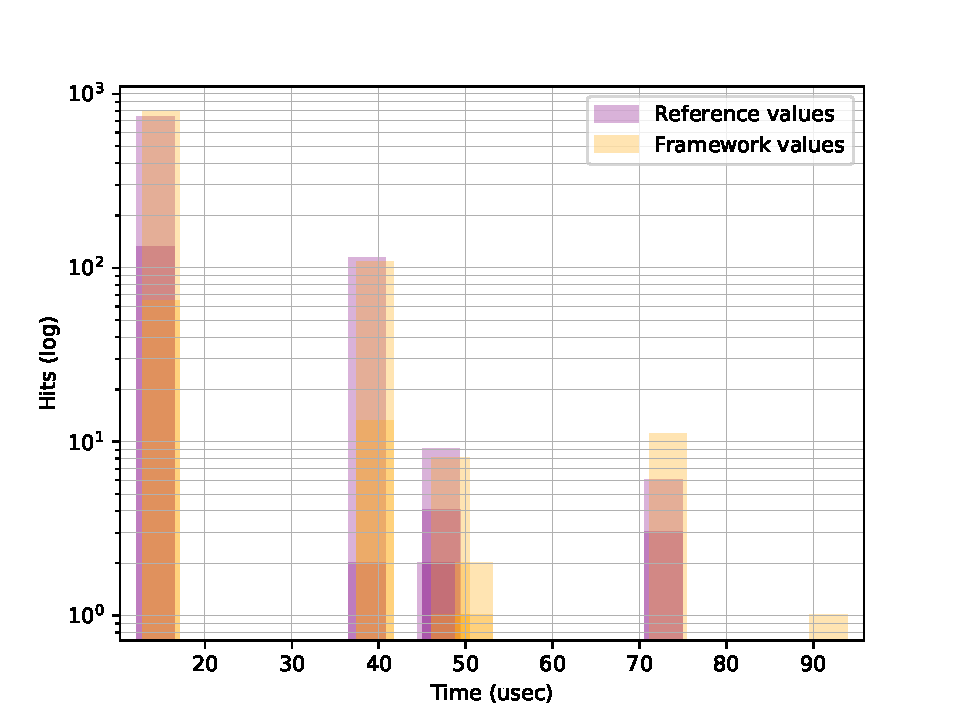
\includegraphics[scale=.7]{assets/comparison-devices-framework-contiki-remote.pdf}
  \caption{distributions comparison with Contiki on the RE-Mote board\label{fig:comparison-devices-framework-contiki-remote}}
\end{figure}

The figure \ref{fig:comparison-devices-framework-contiki-z1} shows the distributions comparison with measurements made on the Z1 board.

\begin{figure}[!ht]
  \centering
  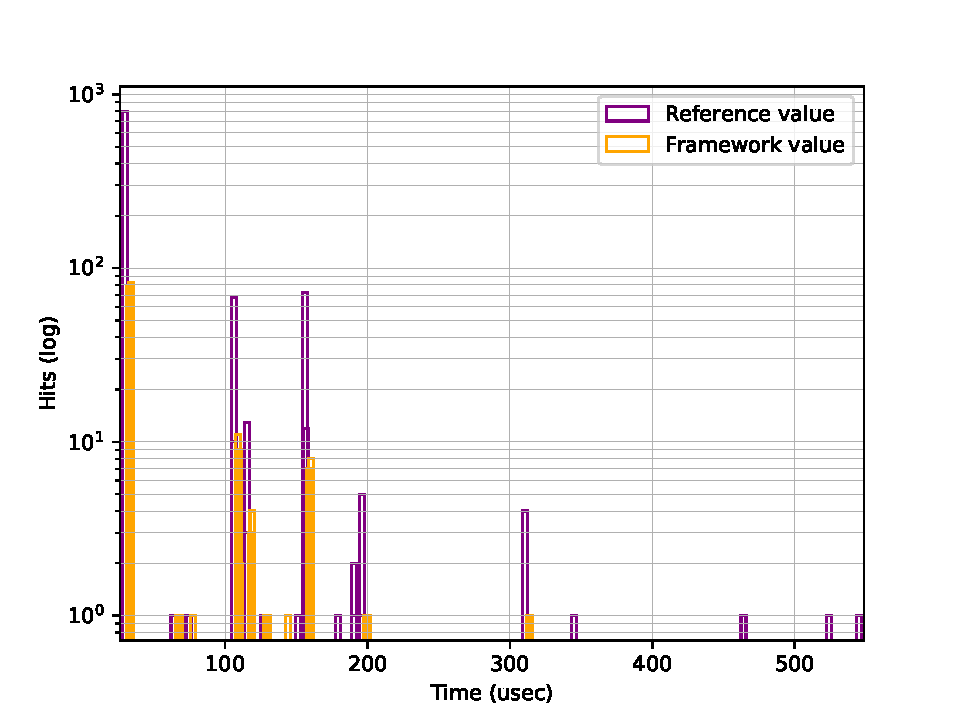
\includegraphics[scale=.7]{assets/comparison-devices-framework-contiki-z1.pdf}
  \caption{distributions comparison with Contiki on the Z1 board\label{fig:comparison-devices-framework-contiki-z1}}
\end{figure}

With RIOT, we have a maximum difference of 3 $\mu$s.
With the RE-Mote board, the difference between the real context switching time and the measurements made by the framework is 0.35 $\mu$s.
In the other hand, with the Z1 board, this difference is 2.99 $\mu$s.
We were not able to determine from where this difference comes from.
However, by comparing the measurements distributions, we see a strong correlation between the reference measurements and the framework measurements.

The figure \ref{fig:devices-comparison-riot-remote} shows the distributions comparison with measurements made on the RE-Mote board and the figure \ref{fig:devices-comparison-riot-z1} shows the same comparison but on the Z1 board.

\begin{figure}[!ht]
  \centering
  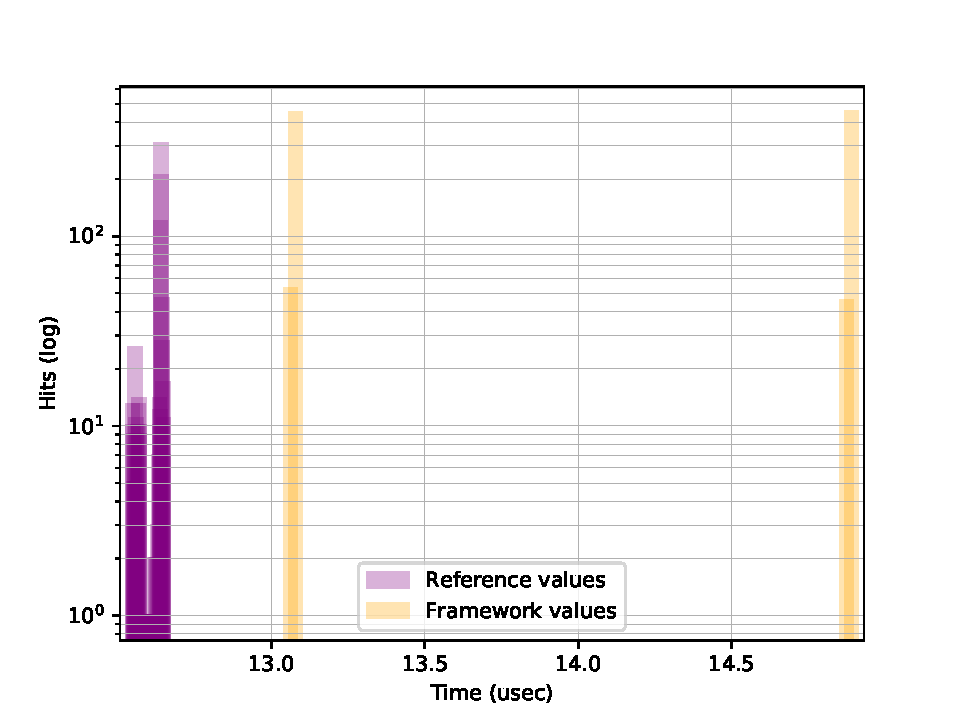
\includegraphics[scale=.7]{assets/comparison-devices-framework-riot-remote.pdf}
  \caption{distributions comparison with RIOT on the RE-Mote board\label{fig:devices-comparison-riot-remote}}
\end{figure}

\begin{figure}[!ht]
  \centering
  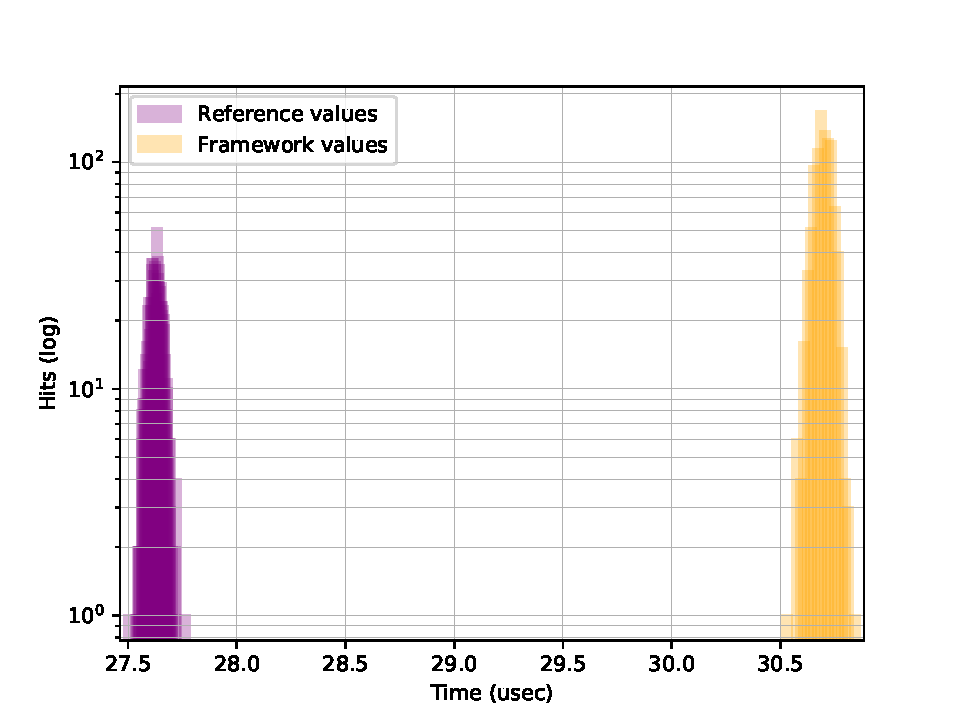
\includegraphics[scale=.7]{assets/comparison-devices-framework-riot-z1.pdf}
  \caption{distributions comparison with RIOT on the Z1 board\label{fig:devices-comparison-riot-z1}}
\end{figure}
\section{Devices framework measurement offset with RIOT}

We notice that the mesures distributions with RIOT are the same between the reference values and the devices framework mesures.
However, the distributions are shifted to the left by an offset as shown by the figure \ref{fig:devices-comparison-riot}.
With the RE-Mote board this offset is $1.35 \mu s$ and with the Z1 board, it is $2.99 \mu s$.

\begin{figure}[!ht]
  \centering
  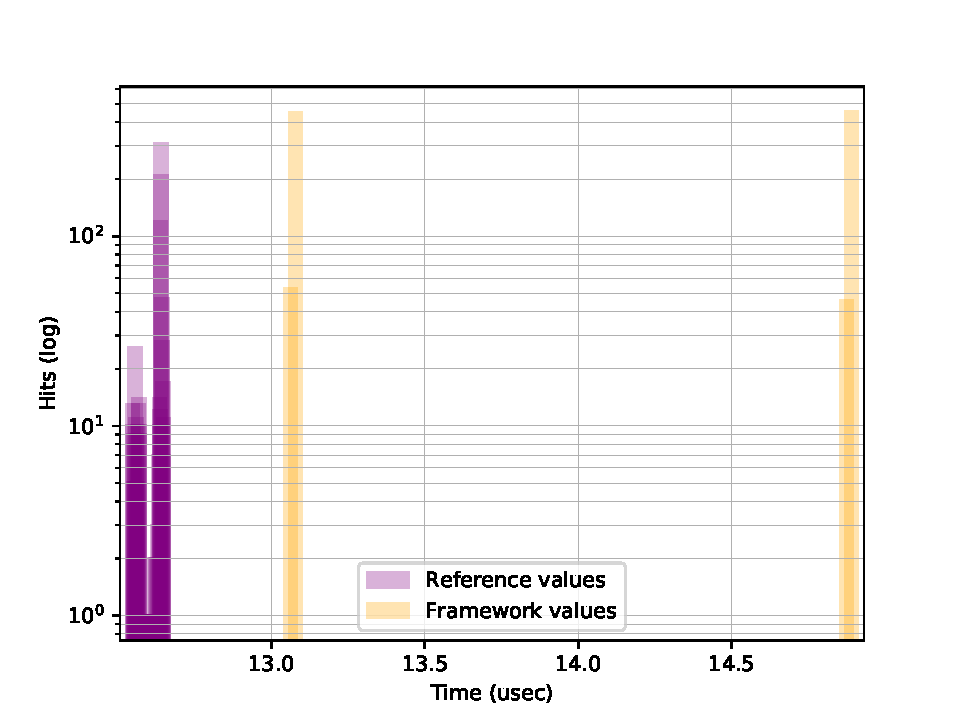
\includegraphics[scale=.7]{assets/comparison-devices-framework-riot-remote.pdf}
  \caption*{Measurements made on the RE-Mote board}
% \end{figure}

% \begin{figure}[!ht]
  \centering
  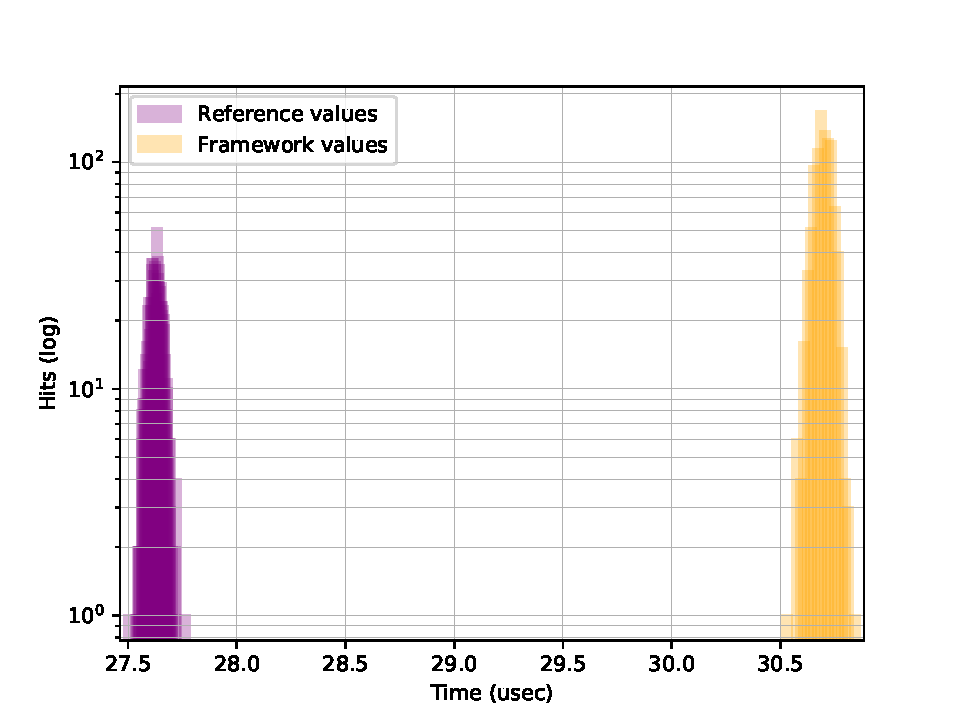
\includegraphics[scale=.7]{assets/comparison-devices-framework-riot-z1.pdf}
  \caption*{Measurements made on the Z1 board}
  \caption{comparison of the devices framework with the reference value on RIOT\label{fig:devices-comparison-riot}}
\end{figure}

\subsection{Causes}

Those offsets can be correlated with the measured overheads.
Indeed, the overheads mesured in the section \ref{sec:overhead} are the same as the offset with RIOT on the two boards.
Our hypothesis is that, with RIOT, there is hidden calls between the user space and the framework space.
\section{Contiki measurements distribution}

By comparing the mesures made with Contiki to the one made with RIOt, we notice a huge difference.
With RIOT, the standard deviation is 31.16ns with the RE-Mote board and 27.61ns with the Z1 board.
With Contiki, the standard deviation is $10\mu s$ with the RE-Mote board and $54\mu s$ with the Z1 board.
The figure \ref{fig:deviation-ref-value} clearly show the difference between the distribution of the reference value between Contiki and RIOT.

\begin{figure}[!ht]
  \centering
  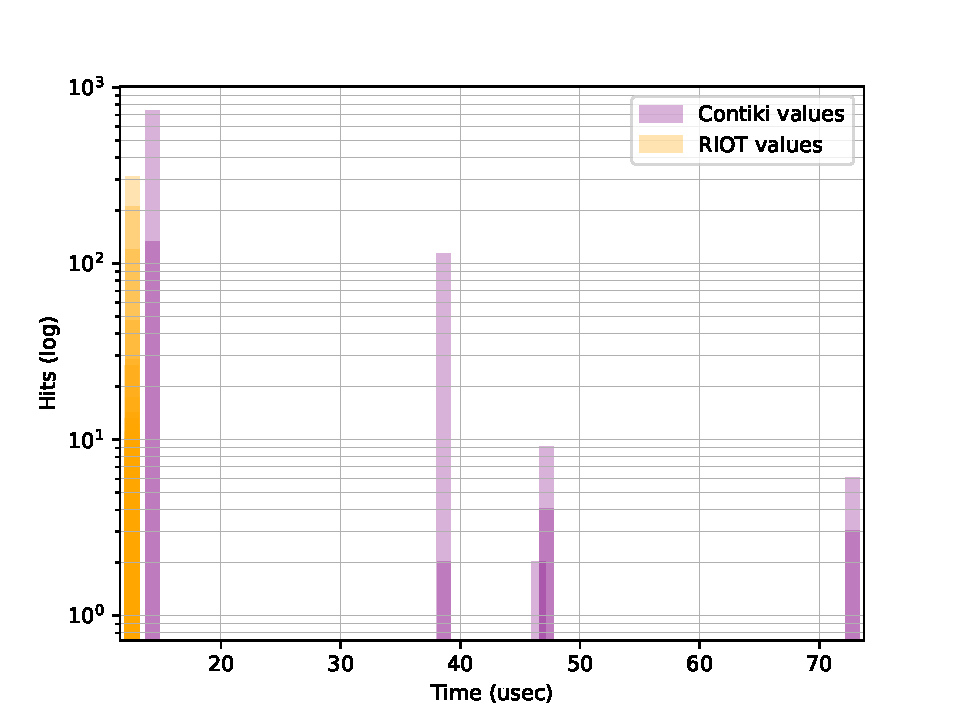
\includegraphics[scale=.7]{assets/offset-remote.pdf}
  \caption*{Mesures made on the RE-Mote board}
  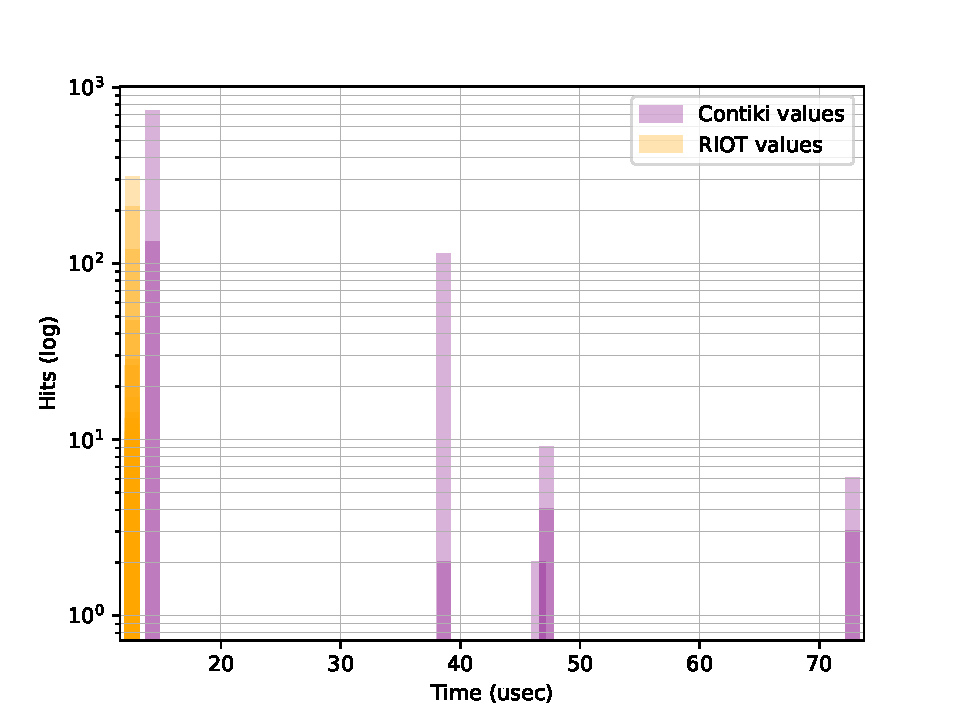
\includegraphics[scale=.7]{assets/offset-remote.pdf}
  \caption*{Mesures made on the Z1 board}
  \caption{distribution comparison between RIOT and Contiki with the reference value\label{fig:deviation-ref-value}}
\end{figure}

At this point, we do not know where this difference comes from.
\section{Summary}

With two RTOS, Contiki and RIOT, and two boards, the RE-mote and the Z1, we have collected data that will define which approach best fits our framework.

With our first approach, we discovered that using the internal real-time clock to compute the context switching time is not suited for our benchmarking framework.
Moreover, outputting measurements to the serial port induce a large overhead that could prevent the benchmarked application to run correctly.

The second approach helps our framework to gather precise measurements.
With the PSLab as the external devices, the framework was able to measure precisely the context switching time on both Contiki and RIOT.

When comparing the distribution of the two approaches to the real context switching time distribution, it is clear that the devices approach is the best fit for our benchmarking framework.

The figure \ref{fig:comparison-all-contiki-remote} and the figure \ref{fig:comparison-all-contiki-z1} show the comparison between the first and the second approach on the RE-mote and the Z1 boards with Contiki.
With a large distribution, it is difficult to see the difference between the reference distribution and the devices approach measurements distribution.
However, we can see that the distribution of the extension approach measurements does not match the distribution of our reference measurements.

\begin{figure}[!ht]
  \centering
  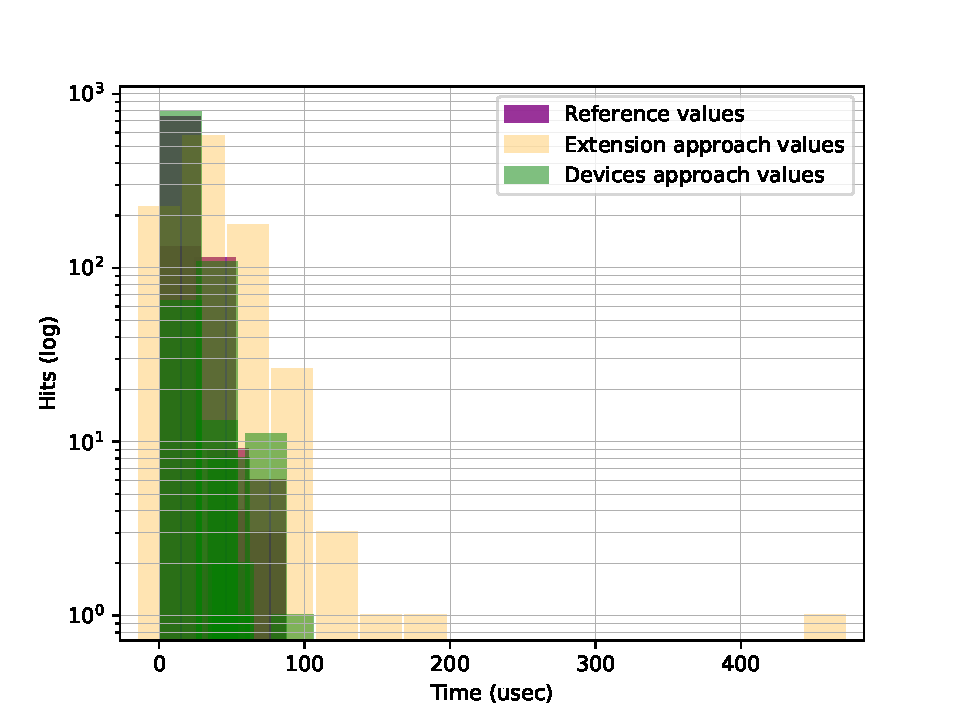
\includegraphics[scale=.7]{assets/comparison-all-contiki-remote.pdf}
  \caption{comparison of the two approaches with Contiki on the RE-Mote board\label{fig:comparison-all-contiki-remote}}
\end{figure}

\begin{figure}[!ht]
  \centering
  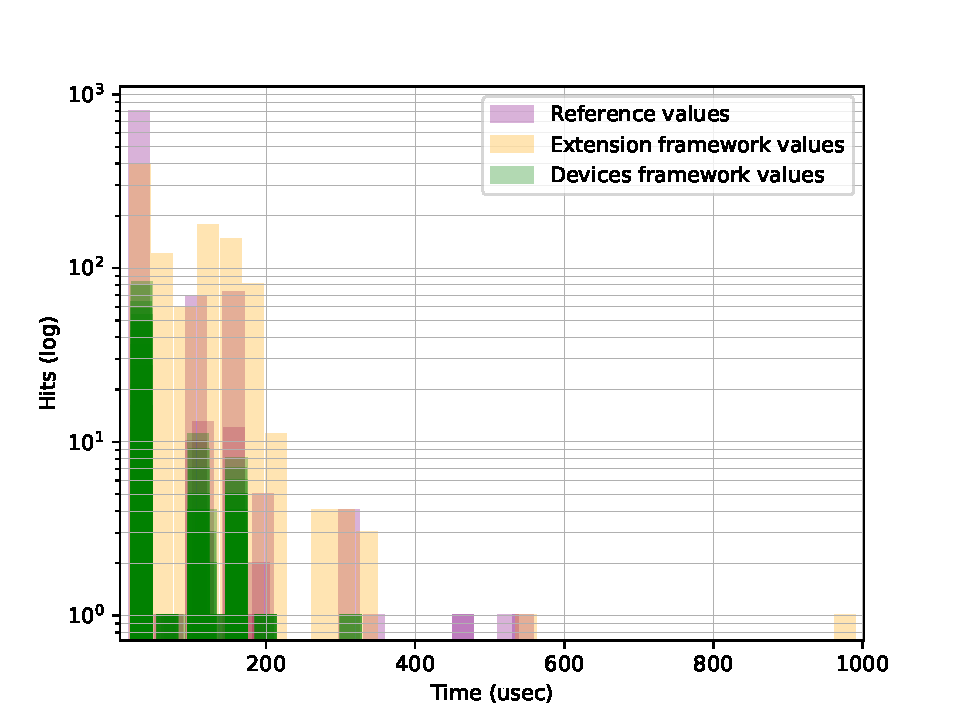
\includegraphics[scale=.7]{assets/comparison-all-contiki-z1.pdf}
  \caption{comparison of the two approaches with Contiki on the Z1 board\label{fig:comparison-all-contiki-z1}}
\end{figure}

The figure \ref{fig:comparison-all-riot-remote} and the figure \ref{fig:comparison-all-riot-z1} show the comparison between the first and the second approach on the RE-mote and the Z1 boards with RIOT.
The devices approach is the closest to the reference measurements.
As the distribution measurements is narrower with RIOT than with Contiki, the difference is more visible.

\begin{figure}[!ht]
  \centering
  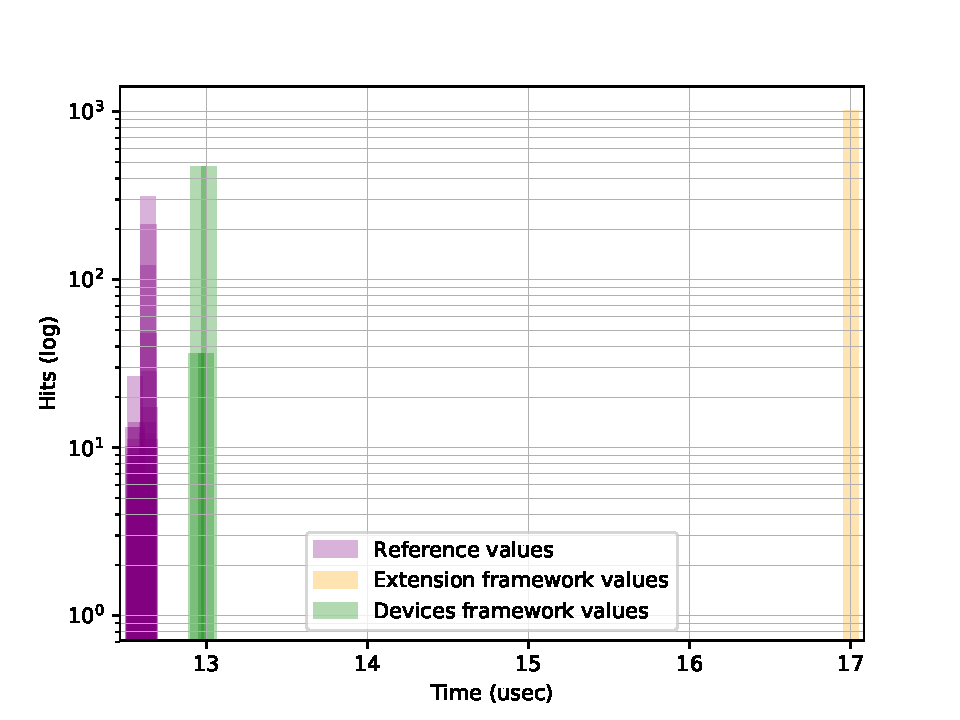
\includegraphics[scale=.7]{assets/comparison-all-riot-remote.pdf}
  \caption{comparison of the two approaches with RIOT on the RE-Mote board\label{fig:comparison-all-riot-remote}}
\end{figure}

\begin{figure}[!ht]
  \centering
  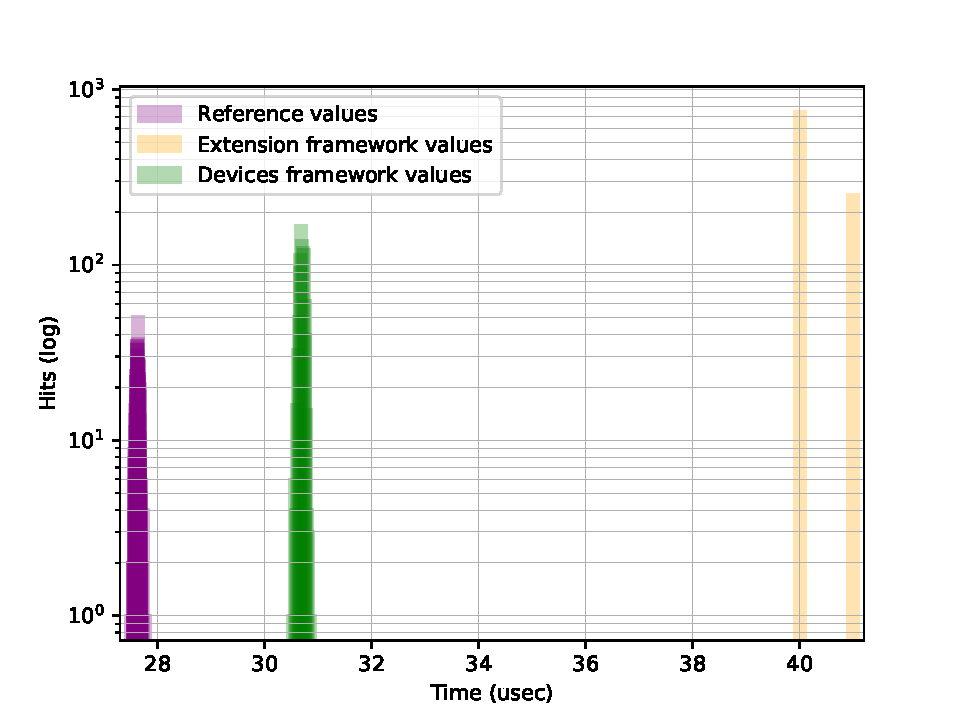
\includegraphics[scale=.7]{assets/comparison-all-riot-z1.pdf}
  \caption{comparison of the two approaches with RIOT on the Z1 board}\label{fig:comparison-all-riot-z1}
\end{figure}


\chapter*{Conclusion and possible improvements}

\section*{First objective}
The first objective of the thesis was to summarize the theory underlying RTOS.
We gathered what we consider the important features in RTOS.
In some points they are similar to general purpose OS but they often implement specificities that are not found in a regular OS.
We presented 3 different embedded OS and compared them from a theoretical point-of-view.

\section*{Second Objective}
The second objective was to develop a proof-of-concept showing to implementing a framework to benchmark RTOS applications is possible.
We had two questions regarding this framework.
The first question was to know if it is possible to build a benchmarking framework capable of performing precise measurements without the use of an oscilloscope.
The second one was to determine if such a framework could be able to retrieve information useful in the context of RTOS.

We started by developing a kernel-integrated framework but it proved more difficult than expected.
This approach was not explored further.

The second approach was to develop a middleware between the RTOS and the application.
This method requires modifications in the application for it to call the framework.
This approach caused a large overhead due to the serial port.
Moreover, it was not able to perform precise measurements.

The third approach was developed with the issues from the second approach in mind.
With the help of the PSLab device, which serves as a monitoring device.
The PSLab benchmarks the board using GPIO and results are collected with a computer connected to the PSLab.
This method brought the best results but an overhead is still observed.

In the end, we can answer our first question in the affirmative.
We were able to implement a framework capable of measuring with enough precision the context switching time of an application running on RTOS.

\subsection*{Going further with the framework}

For our second question, improving the framework is possible.
With the extension approach, it is possible to store more data in a cache while the application runs.
Such information could be the memory usage of the application but also some statistics of the CPU utilization.
It would be possible to determine which task runs the most or which interrupt is called the most.
Those data stored in the cache would be written on the serial port at appropriate times.

Moreover, the PSLab is a customizable tool that can be used to measure the power consumption of the boards.

\cleardoublepage
\pagenumbering{roman}
\listoffigures
\listoftables

%%%%%% Bibliography %%%
\printbibliography

% Back cover page
\backcoverpage
\end{document}